%\documentclass[11pt]{scrartcl}

%
%Packages
%
%%------Ändern von Schriftschnitten - (Muss ganz am Anfang stehen !) ------------
\usepackage{fix-cm}

\usepackage{graphicx}
%\usepackage[
%	a4paper,
%	top=1cm,
%	bottom=2cm,
%	right=2cm,
%	left=2.5cm]{geometry}
\usepackage{booktabs}
\usepackage{ltablex}
\usepackage{nicefrac}
\usepackage[table]{xcolor}
\usepackage[hidelinks]{hyperref}
\usepackage{listings}
\usepackage{tocloft}
%\usepackage{pifont}
\usepackage{pdflscape}
\usepackage{blindtext}
\usepackage{float}
\usepackage{fancyhdr}
\usepackage{enumitem,amssymb}
\usepackage{caption}



%------Einfache Definition der Zeilenabstände und Seitenränder------------------
\usepackage{geometry}
\usepackage{setspace}

%------Schriftgrößenanpassung von einzelnen Textpassagen------------------------
\usepackage{relsize}

%------Trennlinien in Kopf- und Fusszeile
%\usepackage[headsepline, footsepline, ilines]{scrpage2}

%------Grafiken und Farben -----------------------------------------------------
\usepackage{xcolor}
\usepackage{graphicx}

%------Packet zum Sperren, Unterstreichen und Hervorheben von Texten------------
\usepackage{soul}

%------ergänzende Schriftart----------------------------------------------------
\usepackage{helvet}

%------Lange Tabellen-----------------------------------------------------------
%\usepackage{longtable}
%\usepackage{array}
%\usepackage{ragged2e}
%\usepackage{lscape}







%Hier sind alle Einstellungen enthalten, die sich auf das Seiten- und
%Dokumentenlayout beziehen

\documentclass[
  11pt,                   % Schriftgröße
  %DIV12,
  german,                 % für Umlaute, Silbentrennung etc.
  oneside,                % einseitiges Dokument
  titlepage,              % es wird eine Titelseite verwendet
  %parskip=half,           % Abstand zwischen Absätzen (halbe Zeile)
  %headings=normal,        % Größe der Überschriften verkleinern
  %captions=tableheading,  % Beschriftung von Tabellen unterhalb ausgeben
  final                   % Status des Dokuments (final/draft)
]{report}               %


%------Ändern von Schriftschnitten - (Muss ganz am Anfang stehen !) ------------
\usepackage{fix-cm}

\usepackage{graphicx}
%\usepackage[
%	a4paper,
%	top=1cm,
%	bottom=2cm,
%	right=2cm,
%	left=2.5cm]{geometry}
\usepackage{booktabs}
\usepackage{ltablex}
\usepackage{nicefrac}
\usepackage[table]{xcolor}
\usepackage[hidelinks]{hyperref}
\usepackage{listings}
\usepackage{tocloft}
%\usepackage{pifont}
\usepackage{pdflscape}
\usepackage{blindtext}
\usepackage{float}
\usepackage{fancyhdr}
\usepackage{enumitem,amssymb}
\usepackage{caption}



%------Einfache Definition der Zeilenabstände und Seitenränder------------------
\usepackage{geometry}
\usepackage{setspace}

%------Schriftgrößenanpassung von einzelnen Textpassagen------------------------
\usepackage{relsize}

%------Trennlinien in Kopf- und Fusszeile
%\usepackage[headsepline, footsepline, ilines]{scrpage2}

%------Grafiken und Farben -----------------------------------------------------
\usepackage{xcolor}
\usepackage{graphicx}

%------Packet zum Sperren, Unterstreichen und Hervorheben von Texten------------
\usepackage{soul}

%------ergänzende Schriftart----------------------------------------------------
\usepackage{helvet}

%------Lange Tabellen-----------------------------------------------------------
%\usepackage{longtable}
%\usepackage{array}
%\usepackage{ragged2e}
%\usepackage{lscape}





      % enthält eingebundene Packete
\usepackage{comment}

%------Seitenränder-------------------------------------------------------------
\geometry{verbose,                     % zeigt die eingestellten Parameter beim
                                       % Latexlauf an
      paper=a4paper,                   % Papierformat
      top=0mm,                        % Rand oben
      left=25mm,                       % Rand links
      right=25mm,                      % Rand rechts
      bottom=25mm,                     % Rand unten
      pdftex                           % schreibt das Papierformat in die
                                       % Ausgabe damit Ausgabeprogramm
                                       % Papiergröße erkennt
  }

%
% Fancyheader
%
\pagestyle{fancy}
\fancyhf{}
\fancyhead[L]{\large\praktikumTitel\\ \small\projektTitel\\[-.75cm]}
\fancyhead[R]{\thepage}
\fancyfoot[C]{\leftmark}

\renewcommand{\headrulewidth}{1pt}
\renewcommand{\headrule}{\hbox to\headwidth{\color{red}\leaders\hrule height \headrulewidth\hfill}}
\renewcommand{\footrulewidth}{1pt}
\renewcommand{\footrule}{\hbox to\headwidth{\color{red}\leaders\hrule height \footrulewidth\hfill}}

\fancypagestyle{plain}{%
	\fancyhf{}%
	\renewcommand{\headrulewidth}{0pt}
	\fancyfoot[c]{\thepage}
}
%%%%

%Seitenlayout
\onehalfspace        % 1,5-facher Abstand

%------Kopf- und Fußzeilen -----------------------------------------------------
%\pagestyle{scrheadings}

%------Kopf- und Fußzeile auch auf Kapitelanfangsseiten ------------------------
%\renewcommand*{\chapterpagestyle}{scrheadings}

%------Schriftform der Kopfzeile -----------------------------------------------
%\renewcommand{\headfont}{\normalfont}

%----Farben
%\definecolor{tuRed}{cmyk}{0.1,1.0,0.8,0.0}

%------Kopfzeile----------------------------------------------------------------
%\setheadsepline{1pt}[\color{tuRed}]
%\setlength{\headheight}{10mm}        % Höhe der Kopfzeile
%\ihead{\large{\textsc{\praktikumTitel}}\\    % Text in der linken Box
%       \small{\projektTitel}}
%\chead{}                            % Text in der mittleren Box

%----Fusszeile
%\setfootsepline{1pt}[\color{tuRed}]
%\cfoot{}                            % Text in mittlerer Box
%\ofoot{\pagemark}                    % Seitenzahl in rechter Box



%------Labels mit eigenem Text für \ref ----------------------------------------
%\makeatletter
%\def\namedlabel#1#2{\begingroup
%#2%
%\def\@currentlabel{#2}%
%\phantomsection\label{#1}\endgroup
%}
%\makeatother

%------Neue Environments -------------------------------------------------------

%\newcommand{\refsetcounter}[2]{\setcounter{#1}{#2}\addtocounter{#1}{-1}\refstepcounter{#1}}
\newlist{todolist}{itemize}{2}
\setlist[todolist]{label=$\square$}


           % Diese Datei enthält alle Layouteinstellungen
\newcommand{\dokumentTitel}{Dokumentation}


\usepackage[english, ngerman]{babel}
%%% Für PDFLatex
%\usepackage[utf8]{inputenc}
%\usepackage[T1]{fontenc}
%%% Für XeLaTeX
\usepackage{fontspec}
%\setmainfont{DejaVu Sans}
%%%
%
%Config und Commands
%
%%% New Commands & Environments
%%%
\newcommand{\apptitle}{Werwolf-Spielleiter}
\newcommand{\xmark}{\ding{55}}

\setlength{\parindent}{0pt}
\setlength{\cftsubsubsecnumwidth}{4em}

\newcommand{\praktikumTitel}{Praktikum Softwaretechnik 2}
\newcommand{\projektTitel}{Werwolf Spielleiter}
\newcommand{\betreuer}{Matthias Hamann}

\definecolor{tuRed}{cmyk}{0.1,1.0,0.8,0.0}

\newenvironment{packed_itemize}{
	\begin{itemize}
		\setlength{\itemsep}{1pt}
		\setlength{\parskip}{0pt}
		\setlength{\parsep}{0pt}
	}{\end{itemize}}

%%% Default Settings for Listings
\lstset{
	language=Java,
	breaklines=true,
	backgroundcolor=\color{lightgray},
	captionpos=b,
	basicstyle=\small,
	numbers=left,
	numberstyle=\tiny,
	frame=TRbl,
}

\begin{document}

\begin{titlepage}
	\centering
	
	%
	% Logo
	%
	
\includegraphics[width=\textwidth]{titlepage/thl_logo.png}
	
	%
	% Headings
	%
	{\huge \textsc{\praktikumTitel}}\\[0.5cm]
	{\LARGE \textsc{\projektTitel}}\\[1.0cm]
	{\large Sommersemester 2020}\\[1.0cm]
	{\LARGE \bfseries\dokumentTitel}\\[1.0cm]
	%
	% Auftraggeber
	%
	Auftraggeber\\
	Technische Hochschule Lübeck\\
	Betreuer: \betreuer\\
	%
	% Team
	%
	\vfill
	Teammitglieder:\\[0.5cm]
	% ----Tabelle der Praktikumsteilnehmer------------------------------------------
\begin{tabular}{l<{\hspace{20mm}} l<{\hspace{30mm}}}
  Name                   &   E-Mail-Adresse\\      % Zeilenüberschift
  \hline                    % Linie unterhalb der Zeilenüberschrift
  %----Nachfolgend alle Namen und E-Mail-Adressen der Teilnehmer einfügen
  Eric De Ron & eric.ron@stud.th-luebeck.de\\
  Janik Dohrmann & janik.dohrmann@stud.th-luebeck.de\\
  Alonso Essenwanger & alonso.essenwanger@stud.th-luebeck.de\\
  Matthias Hinrichs & matthias.hinrichs@stud.th-luebeck.de\\
  Henrik Möhlmann & henrik.moehlmann@stud.th-luebeck.de\\
  Florian Müller & f.mueller@stud.th-luebeck.de\\
\end{tabular}
%Zur Vereinheitlichung sollten hier die TH Lübeck Emailadressen benutzt werden. % enthält Tabelle der Praktikumsteilnehmer
	\vfill
	Lübeck, \today
\end{titlepage}
%% Dies ist die Titelseite.
% Die Ausgabe darf 1 Seite nicht überschreiten, also ggf. Abstände anpassen
% Die Angabe in [...] gibt den Abstand nach der entsprechenden Zeile an.


%----Stil dieser Seite----------------------------------------------------------
%\thispagestyle{plain}      % Kopfzeile bleibt leer


%----Beginn der Titelseite------------------------------------------------------
\begin{titlepage}

%\hspace*{-2cm}


\includegraphics[width=\textwidth]{titlepage/thl_logo.png}


\vspace*{-2.8cm}


~\\[5ex]

%----zentrierte Ausrichtung über die gesamte Seite----------------------------
\begin{center}

%----Titel des Praktikum (\praktikumTitel in newComments zu verändern)--------
{\relsize{4}{{\textsc{\praktikumTitel}}}}\\[5ex]
%\textsc{\huge \praktikumTitel}\\[5ex]

%----Titel des Teilprojektes (\projektTitel in newComments verändern)---------
{\relsize{3}{{\textsc{\projektTitel}}}}\\[5ex]
%\textsc{\LARGE \projektTitel}\\[5ex]

%Software-Entwicklungspraktikum (SEP)\\
Sommersemester 2020\\[6ex]
%\the\year\\[6ex]

{\relsize{3}{{\bfseries \dokumentTitel}}}\\[5ex]

%----Daten des Auftraggebers
Auftraggeber\\
Technische Hochschule Lübeck\\

Betreuer: \betreuer\\[5ex]

\vspace*{2.8cm}

Teammitglieder:\\

% ----Tabelle der Praktikumsteilnehmer------------------------------------------
\begin{tabular}{l<{\hspace{20mm}} l<{\hspace{30mm}}}
  Name                   &   E-Mail-Adresse\\      % Zeilenüberschift
  \hline                    % Linie unterhalb der Zeilenüberschrift
  %----Nachfolgend alle Namen und E-Mail-Adressen der Teilnehmer einfügen
  Eric De Ron & eric.ron@stud.th-luebeck.de\\
  Janik Dohrmann & janik.dohrmann@stud.th-luebeck.de\\
  Alonso Essenwanger & alonso.essenwanger@stud.th-luebeck.de\\
  Matthias Hinrichs & matthias.hinrichs@stud.th-luebeck.de\\
  Henrik Möhlmann & henrik.moehlmann@stud.th-luebeck.de\\
  Florian Müller & f.mueller@stud.th-luebeck.de\\
\end{tabular}
%Zur Vereinheitlichung sollten hier die TH Lübeck Emailadressen benutzt werden. % enthält Tabelle der Praktikumsteilnehmer

\vspace*{2.0cm}

\vfill
Lübeck, \today

\end{center}
\end{titlepage}



\newgeometry{top=25mm, left=25mm, right=25mm, bottom=25mm}

\tableofcontents

\newpage
\listoffigures

\clearpage
\listoftables   

\clearpage
\lstlistoflistings

\chapter{Einleitung und Kontext}

Im Rahmen des Praktikums Softwaretechnik II haben wir eine Spielleiteranwendung für das Rollenspiel \glqq Die Werwölfe von Düsterwald\grqq{} programmiert. 

\medskip
Bei diesem Spiel sitzen die Mitspieler im Kreis. Sie verkörpern in jeder Spielrunde einen Charakter, den sie zu Beginn jeder Spielrunde verteilt bekommen. Dieser ist den anderen Spielern nicht bekannt. Außerdem können sie einen Beruf ausüben, dieser ist, anders als der Charakter, auch den Mitspielern bekannt. \\
Die Charaktere und Berufe dürfen während der Partie verschiedenste Aktionen durchführen. 

\medskip
Die Charaktere haben unterschiedliche Ziele. Charaktere mit gleichem Ziel gehören einer Fraktion an. Ziel einer Fraktion ist es, ihr Gewinnziel zu erreichen. Dann hat die entsprechende Fraktion gewonnen und die Spielrunde endet. 

\medskip
Die Zielgruppe für die Software sind keine Anfänger, die das Spiel noch erlernen wollen. \\
Der Spielleiter sollte bereits einen ersten Überblick über die Regeln haben, bestenfalls bereits eine handvoll Spielrunden geleitet haben. 

\medskip
Da sich der Spielleiter hierbei unter Umständen sehr viel merken muss und dies meist nur mit einer weiteren Person gemeinsam bewerkstelligen kann, soll die Software ihn durch die Partie leiten und ihm diverse Verwaltungsaufgaben abnehmen. Beispielsweise lässt die Software nur regelkonforme Aktionen zu. Außerdem nimmt es dem Spielleiter viele Dinge ab, die sich nun die Software \glqq merkt\grqq{}. An gebotener Stelle wird diese Information dann dem Spielleiter angezeigt. Beispielhaft kann hier das Liebespaar genannt werden. Da der zweite Partner automatisch stirbt, wenn der erste stirbt, muss sich der Spielleiter das Liebespaar nicht mehr merken, da die Software das übernimmt. Sie benachrichtigt auch den Spielleiter, wenn der zweite Partner aus Liebeskummer stirbt. Als weiteres Beispiel ist zu nennen, dass die Software alle Opfer der Charaktere verwaltet. 

\medskip
Als Vorgabe dienen diesem Projekt die Spielanleitungen von \glqq Die Werwölfe von Düsterwald - Der Pakt\grqq{} und \glqq Die Werwölfe von Düsterwald - Die Gemeinde\grqq{}. Dadurch sind beispielsweise die Charaktere und Berufe, der Spielablauf, sowie die Spielregeln ähnlich wie bei einem Lastenheft vorgegeben. 


% Kapitel 2 enthält nur einige Beispiele
%\chapter{Realisierung}
\Blindtext
\newpage
\section{Beispielcode}
%%%% minipage um zu verhinden, dass das Listing durch Figures oder andere floats zerschnitten wird
\begin{minipage}{\linewidth}
\lstinputlisting[language=Java,
	backgroundcolor=\color{lightgray},
	captionpos=b,
	basicstyle=\small,
	numbers=left,
	numberstyle=\tiny,
	frame=TRbl,
	caption=Beispiellisting von JAVA-Code,
	label={lst:example01}]{sections/examples/helloWorld.java}
% Pfade gelten immer von der Hauptdatei aus (Werwolf-Spielleiter-Doku.tex)	
\end{minipage}
%%%% Figures sind floats, LaTeX platziert sie automatisch. Das kann über extra Optionen der figure verhindert werden ( Option [H] aus package float),
%%%% aber da man Figures usw. eh im Text referenzieren muss, reicht es meistens zu prüfen, dass nichts anderes zerschnitten wurde (siehe Codelisting)
\section{Beispielbild}
\begin{figure}[H]
	\centering
	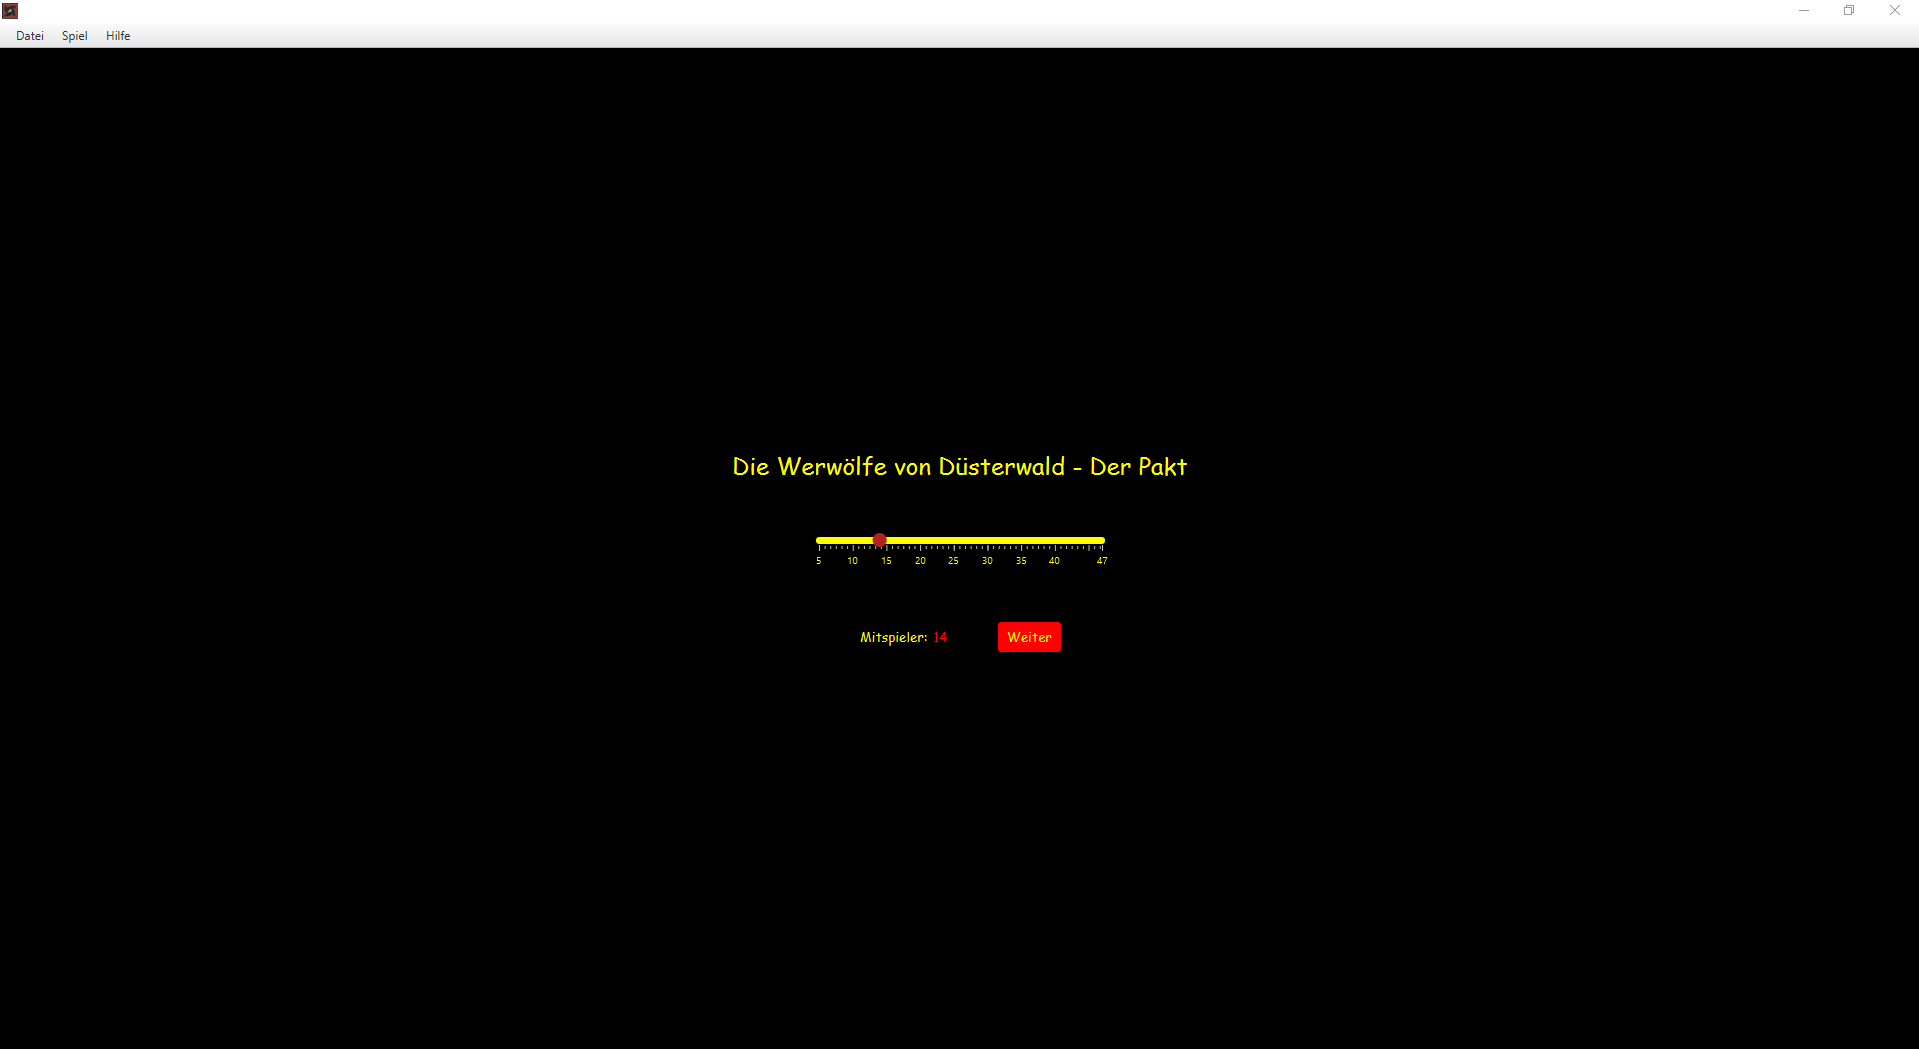
\includegraphics[width=\textwidth]{sections/examples/appStartScreen.png}
	\caption{Startbildschirm des Programms}
	\label{figure:appStartScreen}
\end{figure}
% Beispielreferenzierung auf Element mit label 'figure:appStartScreen'
Wie in Abbildung \ref{figure:appStartScreen} zu sehen...
\chapter{Softwarearchitektur}
Durch die Klasse \textit{SceneManager} wird die Aufbaulogik gesetzt und auch die Reihenfolge, was passiert wenn die entsprechende Szene geladen wird oder wenn diese Szene jetzt erst mal nicht mehr angezeigt werden soll. Im weiterem werden dort auch sehr Elementare Spielregeln gesetzt. Das \textit{Model} hält alle wichtigen Daten, welche für den Spielverlauf wichtig sind. Die \textit{ViewModels} halten die explizierte Logik für jede Szene und die Elementaren Spielregeln der jeweiligen Szene.
 

\section{Model}

\begin{figure}[H]
	\centering
	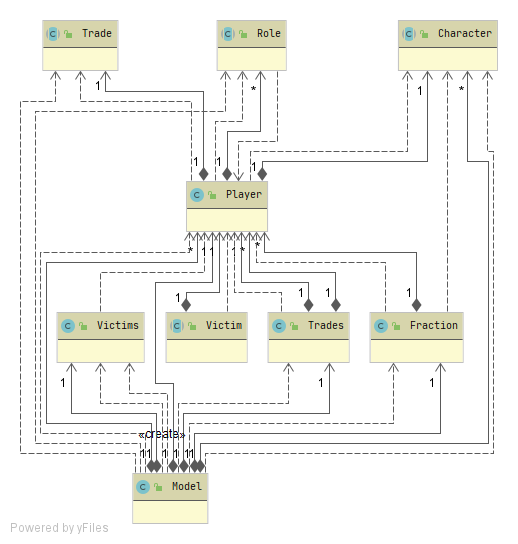
\includegraphics[width=0.8\textwidth]{architektur/model_uml.png}
	\caption{Übersicht Model}
	\label{figure:diagram_model}
\end{figure}

In Abbildung \ref{figure:diagram_model} ist eine grobe Übersicht über das Model zu sehen. Die Hauptklasse des Models ist die Klasse \textit{Model}. Die Klasse \textit{Player} speichert alle relevanten Informationen über einen Spieler ab. Jedem Spieler kann ein Charakter (\textit{Character}), sowie ein Beruf (\textit{Trade}) zugeordnet sein. Für Aktionen des Spielers können ihm mehrere Rollen (\textit{Role}) zugeordnet sein. Die Klasse \textit{Fraction} speichert die Fraktionen der Spieler. Die Klasse \textit{Trades} speichert die Spieler anhand ihres Berufes. Die Klasse \textit{Victims} speichert die Opfer der einzelnen Charaktere. Jede dieser Klassen befindet sich jeweils in einem gleichnamigen Package.

\medskip
Die Klassen \textit{Character}, \textit{Role}, \textit{Trade} und \textit{Victim} sind abstrakt, um für die unterschiedlichen Implementierungen der verschiedenen Charaktere, Rollen, Berufe und Opfer eine einheitliche Ansprache zu gewährleisten, indem diese hiervon abgeleitet werden. Die Klassen \textit{Fraction} und \textit{Trades} sind als Singletons realisiert.

\medskip
In den folgenden Unterkapiteln werden die einzelnen Packages des Models betrachtet. 

\subsection{Model (Package)}
Die Klasse \textit{Model} ist die Hauptklasse des Models. Innerhalb dieses Unterkapitels wird im Folgenden mit Model jeweils die Klasse und nicht das gesamte Model bezeichnet. 
Hier werden die allgemeinen Daten für eine Spielrunde abgespeichert. Außerdem erfolgt hierüber der Zugriff auf einige weitere Objekte, die beispielsweise die Opfer oder die Fraktionen verwalten. 

Es werden zunächst die Attribute des Models betrachtet.

\medskip
\begin{center}
	\begin{minipage}{0.7\textwidth}
		\lstinputlisting[firstnumber=19, firstline=19, lastline=36, caption=Model Attribute (1), label= lst:modelAttribute01]{../src/main/java/de/werwolf_spielleiter/model/Model.java}
	\end{minipage}
\end{center}


In \autoref{lst:modelAttribute01} sind die Attribute zu sehen, die Anzahlen abspeichern. Das Attribut \textit{countPlayer} speichert die Anzahl der Mitspieler. Die weiteren Attribute speichern jeweils die Anzahl der jeweiligen Charaktere. Das Attribut \textit{countWerewolf} speichert beispielsweise die Anzahl der Werwölfe. 

\medskip
\begin{center}
	\begin{minipage}{0.7\textwidth}
		\lstinputlisting[firstnumber=38, firstline=38, lastline=48, caption=Model Attribute (2), label= lst:modelAttribute02]{../src/main/java/de/werwolf_spielleiter/model/Model.java}
	\end{minipage}
\end{center}

In \autoref{lst:modelAttribute02} sind zunächst die Attribute des Hauptmanns zu sehen. Das Attribut \textit{sheriff} speichert ab, ob mit Hauptmann gespielt wird. Die Attribute \textit{sheriffWasVote} und \textit{nextSheriffVote} speichern ab, ob bereits ein Hauptmann gewählt wurde, bzw. ob ein Nachfolger als Hauptmann bestimmt werden muss. 
Das Attribut \textit{hunterPhase} speichert ab, ob der Jäger sich ein Opfer suchen muss. 
Das Attribut \textit{greatWolfInfected} speichert ab, ob der Urwolf bereits ein Werwolf Opfer infiziert hat. 
Das Attribut \textit{werewolfDead} speichert ab, ob bereits ein Werwolf* \footnote{Werwolf in beliebiger Gestalt: einfacher Werwolf, Urwolf, Großer, böser Wolf, Weißer Werwolf, Wildes Kind als Wolf, Wolfshund als Wolf, infiziertes Werwolf Opfer} getötet wurde. 

\medskip
\begin{center}
	\begin{minipage}{0.7\textwidth}
		\lstinputlisting[firstnumber=50, firstline=50, lastline=55, caption=Model Attribute (3), label= lst:modelAttribute03]{../src/main/java/de/werwolf_spielleiter/model/Model.java}
	\end{minipage}
\end{center}

In \autoref{lst:modelAttribute03} sind die Attribute bezüglich der Berufe zu sehen. 
Das Attribut \textit{playWithTrade} speichert ab, ob mit Berufen gespielt wird. Die drei nachfolgenden Attribute speichern die jeweilige Anzahl der verschiedenen Berufe. Das Attribut \textit{countVagabond} speichert beispielsweise die Anzahl der Vagabunden. Das Attribut \textit{allowConfession} gibt zu jedem Zeitpunkt Auskunft darüber, ob der Beichtvater gerade seine Aktion ausführen darf. 

\medskip
\begin{center}
	\begin{minipage}{0.7\textwidth}
		\lstinputlisting[firstnumber=57, firstline=57, lastline=67, caption=Model Attribute (4), label= lst:modelAttribute04]{../src/main/java/de/werwolf_spielleiter/model/Model.java}
	\end{minipage}
\end{center}

Die ersten beiden Attribute in \autoref{lst:modelAttribute04} speichern jeweils die Liste aller Spieler, bzw. die Liste aller lebenden Spieler. 
Das Attribut \textit{cardThiefList} speichert die beiden Charaktere für den Dieb. 
Das Attribut \textit{night} speichert ab, ob gerade Tag oder Nacht ist. Ist es \textit{false}, ist gerade Tag. 
Das Attribut \textit{day} speichert die Anzahl der Tage, die seit Beginn der Spielrunde verstrichen sind. Begonnen wird mit der Zählung bei eins. 

\medskip
\begin{center}
	\begin{minipage}{0.7\textwidth}
		\lstinputlisting[firstnumber=69, firstline=69, lastline=79, caption=Model Attribute (5), label= lst:modelAttribute05]{../src/main/java/de/werwolf_spielleiter/model/Model.java}
	\end{minipage}
\end{center}

In Abbildung \autoref{lst:modelAttribute05} sind zunächst einige weitere Objekte gespeichert, die Teile des Spiels verwalten. Das Attribut \textit{fraction} speichert die Referenz auf das Objekt, das die Fraktionen der Spieler verwaltet. 
Das Attribut \textit{trades} speichert die Referenz auf das Objekt, das die Berufe der Spieler verwaltet. 
Das Attribut \textit{victims} speichert die Referenz auf das Objekt, das die Opfer der Charaktere verwaltet. 
Das Attribut \textit{idolWildChild} speichert die Referenz auf den Spieler, der das Vorbild des Wilden Kindes ist. 

\begin{figure}[H]
	\centering
	\includegraphics[width=0.75\textwidth]{architektur/model_methods.pdf}
	\caption{Model Methoden}
	\label{figure:model_methods}
\end{figure}

In Abbildung \ref{figure:model_methods} sind die Methoden des Models dargestellt. Die \textit{get} und \textit{set} Methoden, sowie Methoden um die \textit{boolean} Attribute abzufragen oder zu setzen, wurden hier der Übersichtlichkeit wegen nicht aufgeführt. Zu fast jeder Variable gibt es solche Methoden.

\medskip
Die Methode \textit{resetModel(): void} setzt das Model für eine neue Spielrunde zurück. \\
Die Methode \textit{getCharsStack(): List<Character>} liefert anhand der gespeicherten Anzahlen der Charaktere eine Liste mit Charakter Objekten. In dieser Liste kommt jeder Charakter anhand seiner gespeicherten Anzahl vor.

\medskip
Die Methode \textit{startGame(): void} startet eine Spielrunde. Zunächst werden alle Spieler zur Liste der lebenden Spieler hinzugefügt. Es wird die Methode \textit{getCharsStack()} aufgerufen, um eine Liste mit Charakteren zu bekommen.
Anschließend wird jedem Spieler aus dieser Liste zufällig ein Charakter zugeteilt. Dazu bekommt er die entsprechenden Rollen. Außerdem wird er seiner Fraktion (passend zur Charakterkarte) zugeordnet. 
Wird mit Berufen gespielt, wird danach jedem Spieler zufällig ein Beruf zugeteilt. 
Ist einem der Spieler der Dieb als Charakter zugeteilt worden, werden abschließend die zwei Charaktere für den Dieb zufällig aus der anfangs erhaltenen Liste mit Charakteren ausgewählt. 

\medskip
Die Methode \textit{getTradeStack(): List<Trade>} liefert anhand der gespeicherten Anzahlen der Berufe eine Liste mit Trade Objekten. In dieser Liste kommt jeder Beruf anhand seiner gespeicherten Anzahl vor. 

\medskip
Die Methode \textit{startNight(): void} startet die Nacht. Die Variable für die Nacht (\textit{night}) wird auf \textit{true} gesetzt. Die Variable für die Tage (\textit{dax}) wird inkrementiert. Abschließend wird das \textit{Victims} Objekt zurückgesetzt. 

\medskip
Die Methode \textit{initPlayerList(size: int): void} setzt die Spieleranzahl (\textit{countPlayer}) auf die übergebene Anzahl. Außerdem wird die Liste aller Spieler als leere Liste initialisiert, falls sie das noch nicht ist. 

\medskip
Die Methode \textit{isRoleInGame(role: Role): boolean} prüft, ob ein lebender Spieler die übergebene Rolle hat. Ist das der Fall, wird \textit{true} zurückgegeben, andernfalls \textit{false}. 

\medskip
Die Methode \textit{getFirstPlayerWithRole(role: Role): Player} gibt den ersten Spieler aus der Liste der lebenden Spieler zurück, der die übergebene Rolle hat. Hat kein Spieler diese Rolle, wird \textit{null} zurückgegeben. 

\medskip
Die Methode \textit{addPlayer(player: Player): boolean} fügt den übergebenen Spieler der Liste aller Spieler hinzu, wenn die Referenz nicht \textit{null} ist. Im letzteren Fall ist der Rückgabewert \textit{false}, andernfalls \textit{true}. 

\medskip
Die Methode \textit{die(player: Player): boolean} lässt einen übergebenen Spieler sterben, wenn die Referenz nicht \textit{null} ist. Dabei wird der Spieler aus der Liste der lebenden Spieler entfernt. Außerdem wird das \textit{Fraction} Objekt angewiesen, den Spieler zu entfernen, sowie der Spieler aus dem \textit{Trades} Objekt entfernt. War der Spieler ein Werwolf, wird gespeichert, dass bereits ein Werwolf gestorben ist. Abschließend wird der Spieler angewiesen, sich selbst sterben zu lassen. Ist der übergebene Spieler \textit{null}, ist der Rückgabewert \textit{false}, andernfalls ist er \textit{true}. 

\medskip
Die Methode \textit{changeThiefToNewCharacter(player: Player, newCharacter: Character): boolean} setzt dem Dieb (\textit{player}) den übergebenen Charakter (\textit{newCharacter}) als neuen Charakter. 
Dabei wird der Dieb zunächst aus dem \textit{Fraction} Objekt entfernt. Danach wird ihm der neue Charakter, sowie die zugehörigen Rollen gesetzt. Abschließend wird er wieder dem \textit{Fraction} Objekt hinzugefügt und dabei automatisch der richtigen Fraktion zugeordnet. Ist eine der übergebenen Referenzen \textit{null}, ist der Rückgabewert \textit{false}, andernfalls ist er \textit{true}.  

\subsection{Player}

Die Klasse \textit{Player} repräsentiert einen Spieler innerhalb einer Spielrunde. Dafür existieren folgende Attribute: 

\medskip
\begin{center}
	\begin{minipage}{0.7\textwidth}
		\lstinputlisting[firstnumber=21, firstline=21, lastline=29, caption=Player Attribute, label= lst:playerAttribute]{../src/main/java/de/werwolf_spielleiter/player/Player.java}
	\end{minipage}
\end{center}

Das Attribut \textit{name} speichert den Namen des Spielers. 
Das Attribut \textit{status} speichert den Status des Spielers. Dies kann beispielsweise \textit{alive} oder \textit{dead} sein. 
Das Attribut \textit{characterCardBack} speichert die Rückseite der Charakterkarte. 
Das Attribut \textit{characterCardFront} speichert die Vorderseite der Characterkarte. 
Das Attribut \textit{characterCardProperty} speichert die aktuell angezeigte Seite der Characterkarte. 
Das Attribut \textit{awake} speichert, ob der Spieler gerade aufgewacht ist, oder schläft. Wichtig ist dieses Attribut nur nachts, da tagsüber eh alle Spieler wach sind. 
Das Attribut \textit{character} speichert den Charakter, den der Spieler in der Spielrunde verkörpert. 
Das Attribut \textit{rolesList} speichert alle Rollen des Spielers. 
Das Attribut \textit{trade} speichert den Beruf des Spielers. Hat er keinen, ist dieses Attribut \textit{null}. 

\medskip
\begin{figure}
	\centering
	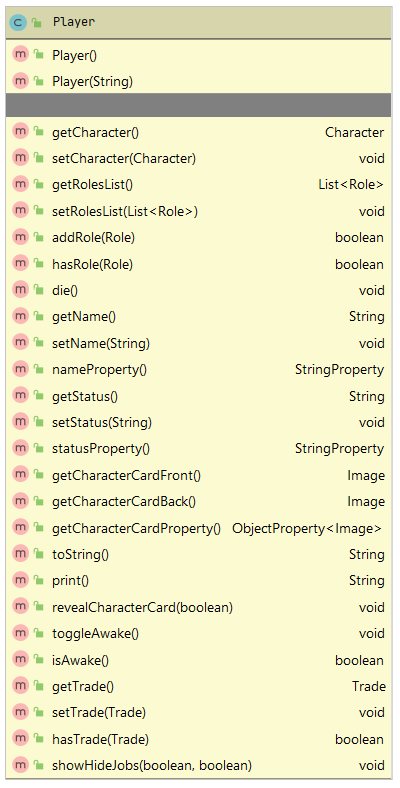
\includegraphics[width=9cm]{architektur/player_methods.png}
	\caption{Player Methoden}
	\label{figure:player_methods}
\end{figure}

Wie in \autoref{figure:player_methods} zu sehen, besitzt Player zwei Konstruktoren. Zunächst einen Konstruktor ohne Variablen. Dieser ist dazu da, den Spieler schon einmal anzulegen, ohne dass der Nutzer bereits einen Namen eingegeben haben muss. Der zweite bekommt einen String übergeben. Dies ist der Name des anzulegenden Spielers. 

\medskip
Weiterhin stehen diverse \textit{get} und \textit{set} Methoden zur Verfügung, um den Spieler zu manipulieren. 

\medskip
Die Methode \textit{addRole(role: Role): boolean} fügt dem Spieler die übergebene Rolle hinzu, falls er die Rolle noch nicht hat. In diesem Fall ist der Rückgabewert \textit{true}. Hat der Spieler die Rolle bereits, wird sie nicht noch einmal hinzugefügt und der Rückgabewert ist \textit{false}. 

\medskip
Die Methode \textit{hasRole(r: Role): boolean} gibt Aufschluss darüber, ob der Spieler die übergebene Rolle besitzt. In dem Fall ist der Rückgabewert \textit{true}. Besitzt er die Rolle nicht, ist der Rückgabewert \textit{false}. 

\medskip
Die Methode \textit{die(): void} lässt den Spieler sterben. Dazu setzt sie den Status auf \textit{dead}. 

\medskip
Die Methode \textit{toString(): String} gibt den Namen des Spielers zurück. 

\medskip
Die Methode \textit{print(): String} liefert eine etwas ausführlichere String Representation als \textit{toString()}. 

\medskip
Die Methode \textit{revealCharacterCard(reveal: boolean): void} setzt die aktuell angezeigte Seite der Charakterkarte. Ist der übergebene Wert \textit{true}, so wird die Vorderseite gesetzt, andernfalls die Rückseite. 

\medskip
Die Methode \textit{toggleAwake(): void} invertiert den Erwachenszustand. 

\medskip
Die Methode \textit{hasTrade(trade: Trade): boolean} gibt Aufschluss darüber, ob der Spieler den übergebenen Beruf hat. In dem Fall ist der Rückgabewert \textit{true}. Hat er den Beruf nicht, ist der Rückgabewert \textit{false}. 

\medskip
Die Methode \textit{showHideJobs(jobsRevealed: boolean, cardsRevealed: boolean): void} setzt das Bild der Charakterkarte entsprechend den beiden übergebenen Werte für den aktuellen Soll-Zustand der Karten. Ist \textit{jobsRevealed} \textit{true}, so wird das Berufsicon gesetzt. Ist \textit{jobsRevealed} \textit{false}, so wird die Vorderseite der Charakterkarte gesetzt, wenn \textit{cardsRevealed} \textit{true} ist. Andernfalls wird die Rückseite der Charakterkarte gesetzt. 

\subsection{Character}

\begin{figure}[H]
	\centering
	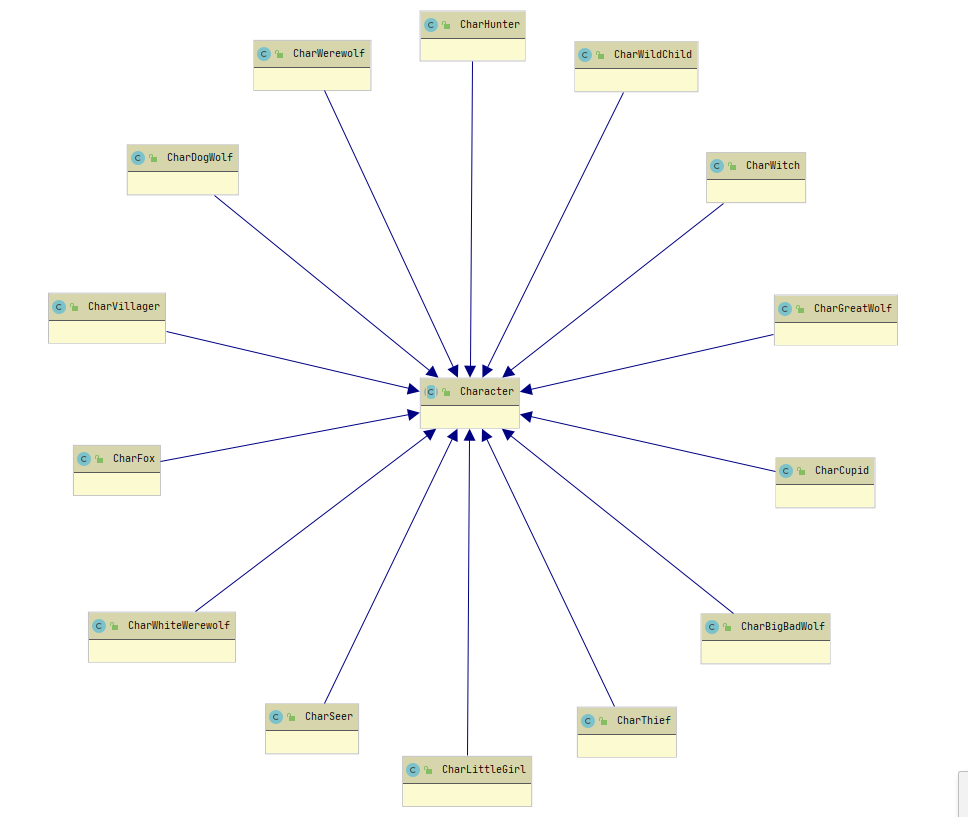
\includegraphics[width=14cm]{architektur/character_uebersicht.png}
	\caption{Character Übersicht}
	\label{figure:character_uebersicht}
\end{figure}

Alle Charaktere sind von der abstrakten Klasse \textit{Character} abgeleitet, wie in \autoref{figure:character_uebersicht} zu sehen. So ist für jeden Charakter eine einheitliche Ansprache gewährleistet und es können einfach weitere Charaktere implementiert werden. 

\medskip
\begin{center}
	\begin{minipage}{0.7\textwidth}
		\lstinputlisting[firstnumber=10, firstline=10, lastline=12, caption=Player Attribute, label= lst:characterAttribute]{../src/main/java/de/werwolf_spielleiter/character/Character.java}
	\end{minipage}
\end{center}

Wie in \autoref{lst:characterAttribute} zu sehen, hat die Klasse \textit{Character} drei Attribute. Das Attribut \textit{name} speichert den Namen des Charakters. Die Attribute \textit{characterCardBack} und \textit{characterCardFront} speichern die Rück- bzw. Vorderseite der zugehörigen Charakterkarte. 

\begin{figure}[H]
	\centering
	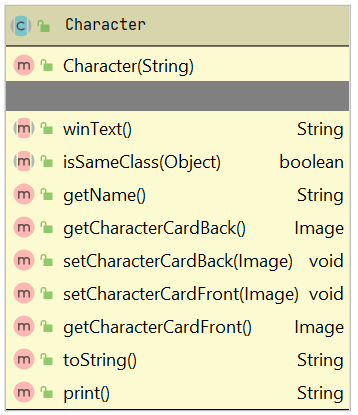
\includegraphics[width=6cm]{architektur/character_methods.png}
	\caption{Character Methoden}
	\label{figure:character_methods}
\end{figure}

Wie in \autoref{figure:character_methods} zu sehen, hat die Klasse \textit{Character} einen Konstruktor. Diesem wird der Name des Charakters übergeben. 

\medskip
Weiterhin gibt es als Schnittstelle für eingangs erwähnte Variablen \textit{get} und \textit{set} Methoden. 

\medskip
Die Methode \textit{toString(): String} liefert eine String Repräsentation des Charakters, die nur den Namen enthält. 
Die Methode \textit{print(): String} liefert eine etwas ausführlichere Repräsentation. 

\medskip
Die Methoden \textit{winText(): String} und \textit{isSameClass(obj Object): boolean} sind abstrakt. Diese werden von den abgeleiteten Klassen unterschiedlich implementiert. 

\medskip
Die meisten Charaktere unterscheiden sich nur in der Implementierung der vorgegebenen abstrakten Methoden und dem Konstruktor. Im Folgenden wird daher beispielhaft ein Charakter vorgestellt und die Unterschiede zu den anderen Charakteren dargelegt. 

\medskip
Die meisten Charaktere haben keine eigenen Attribute, diejenigen mit eigenen Attributen werden später betrachtet. 

\begin{figure}[H]
	\centering
	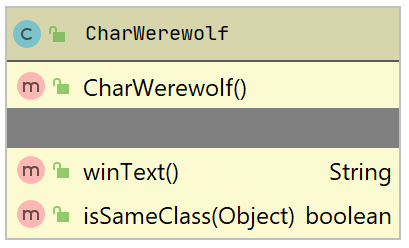
\includegraphics[width=6cm]{architektur/characterWerewolf_methods.png}
	\caption{Charakter Werwolf Methoden}
	\label{figure:characterWerewolf_methods}
\end{figure}

Wie in \autoref{figure:characterWerewolf_methods} zu sehen, wird exemplarisch die Klasse \textit{CharWerwolf} betrachtet. 
Wie erwähnt, erbt die se Klasse von \textit{Character} und hat keine eigenen Attribute. 

\medskip
Der Konstruktor ruft zunächst den Konstruktor von \textit{Character} mit dem Namen des Charakters auf. Anschließend werden die Vorder- und Rückseiten der Charakterkarte gesetzt. 

\medskip
Die Methode \textit{winText(): String} gibt den Text zurück, der angezeigt wird, wenn die Fraktion dieses Charakters gewinnt. 

\medskip
Die Methode \textit{isSameClass(obj: Object): boolean} gibt \textit{true} zurück, wenn das übergebene Objekt eine Instanz der selben Klasse ist, wie der Charakter, folglich also, wenn es derselbe Charakter ist. Andernfalls ist der Rückgabewert \textit{false}. 

\begin{figure}[H]
	\centering
	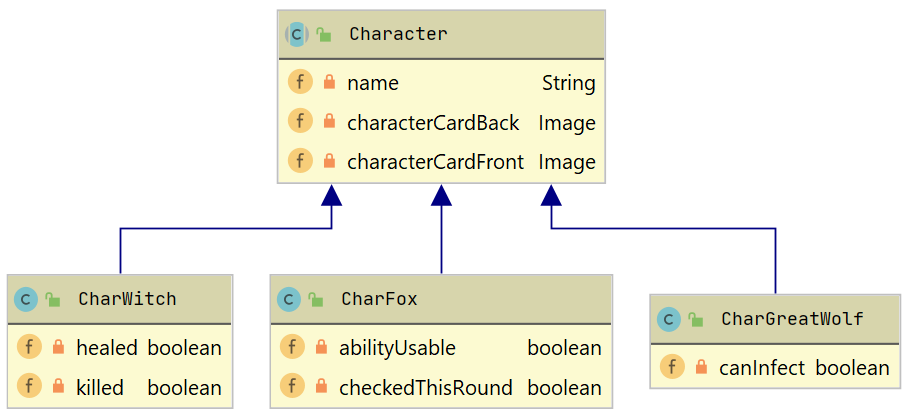
\includegraphics[width=11cm]{architektur/character_extra_attributes.png}
	\caption{Charaktere mit weiteren Attributen}
	\label{figure:character_extra_attributes}
\end{figure}

Wie in \autoref{figure:character_extra_attributes} zu sehen ist, gibt es drei Klassen, die weitere Attribute definiert haben. 

\medskip
Die Klasse \textit{CharWitch} hat die Attribute \textit{healed} und \textit{killed} um jeweils zu speichern, ob der Heiltrank, bzw. der Gifttrank in der Spielrunde schon eingesetzt wurde. Im Fall, dass er eingesetzt wurde, ist der Wert \textit{true}. 

\medskip
Die Klasse \textit{CharFox} hat das Attribut \textit{abilityUsable}, um zu speichern, ob der Fuchs seine Fähigkeit noch nutzen kann. Das Attribut \textit{checkedThisRound} speichert, ob der Fuchs in der aktuellen Nacht schon jemanden überprüft hat. 

\medskip
Die Klasse \textit{CharGreatWolf} hat das Attribut \textit{canInfect}, das speichert, ob der Urwolf noch jemanden infizieren kann. 

\begin{figure}[H]
	\centering
	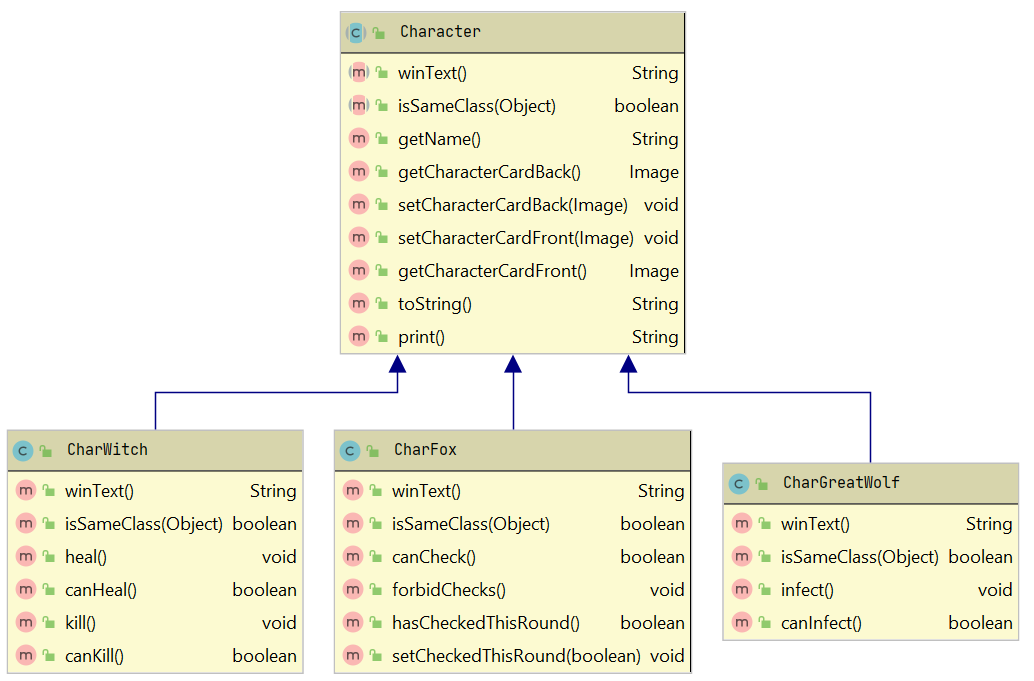
\includegraphics[width=13cm]{architektur/character_extra_methods.png}
	\caption{Charaktere mit weiteren Methoden}
	\label{figure:character_extra_methods}
\end{figure} 

Wie in \autoref{figure:character_extra_methods} zu sehen, haben die drei Klassen \textit{CharWitch}, \textit{CharFox} und \textit{CharGreatWolf} auch weitere Methoden definiert. 

\medskip
In der Klasse \textit{CharWitch} gibt es die Methode \textit{heal(): void} um zu speichern, dass die Hexe den Heiltrank eingesetzt hat. Die Methode \textit{canHeal(): boolean} gibt Auskunft darüber, ob die Hexe den Heiltrank schon eingesetzt hat. 
Die Methode \textit{canKill(): boolean} gibt Auskunft darüber, ob die Hexe den Gifttrank schon eingesetzt hat. 
Die Methode \textit{kill(): void} speichert ab, dass die Hexe den Gifttrank eingesetzt hat. 

In der Klasse \textit{CharFox} gibt es vier weitere Methoden. 
Die Methode \textit{canCheck(): boolean} gibt Aufschluss darüber, ob der Fuchs noch seine Fähigkeit besitzt. 
Die Methode \textit{forbidChecks(): void} entzieht dem Fuchs seine Fähigkeit. 
Die Methode \textit{hasCheckedThisRound(): boolean} gibt Aufschluss darüber, ob der Fuchs in der aktuellen Nacht bereits jemanden überprüft hat. 
Die Methode \textit{setCheckedThisRound(checkedThisRound: boolean): void} setzt den Wert dafür, ob der Fuchs in der aktuellen Nacht bereits jemanden überprüft hat. Ist der übergebene Wert \textit{true}, so hat der Fuchs bereits jemanden überprüft, ist er \textit{false}, so hat der Fuchs in der aktuellen Nacht noch niemanden überprüft. 

\medskip
In der Klasse \textit{CharGreatWolf} gibt es zwei weitere Methoden. 
Die Methode \textit{canInfect(): boolean} gibt Aufschluss darüber, ob der Urwolf seine einmalige Fähigkeit, das Werwolf Opfer zu infizieren, noch besitzt. 
Die Methode \textit{infect(): void} speichert, dass der Urwolf seine einmalige Fähigkeit bereits eingesetzt hat. Damit wird ihm seine einmalige Fähigkeit entzogen. 

\subsection{Role}

\begin{figure}[H]
	\centering
	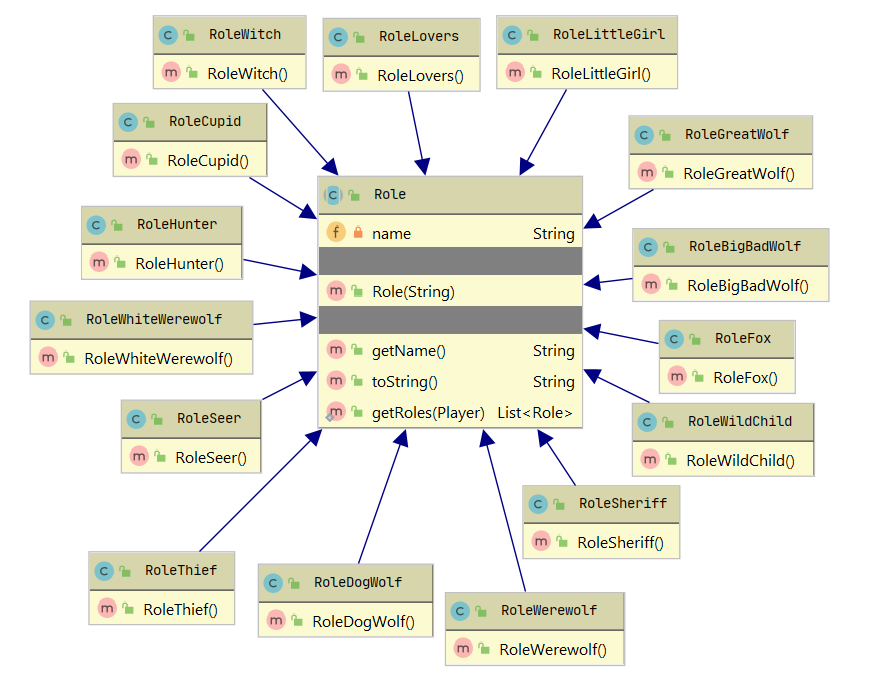
\includegraphics[width=\textwidth]{architektur/role_uml.png}
	\caption{Role Übersicht}
	\label{figure:role_uebersicht}
\end{figure}

Alle Rollen sind von der abstrakten Klasse \textit{Role} abgeleitet, wie in \autoref{figure:role_uebersicht} zu sehen. So ist für jede Rolle eine einheitliche Ansprache gewährleistet und es können einfach weitere Rollen implementiert werden. 

\medskip
Die Klasse \textit{Role} hat einen Konstruktor, der den Namen der Rolle als String übergeben bekommt. 
Der Name ist über die Methode \textit{getName(): String} zugänglich. 

\medskip
Mittels \textit{toString(): String} ist eine String Repräsentation der Rolle zugänglich, die den Namen enthält. 

\medskip
Die statische Methode \textit{getRoles(player: Player): List<Role>} gibt für einen übergebenen Spieler eine Liste mit den zu seinem Charakter gehörenden Rollen zurück. Hat der Spieler keinen Charakter gesetzt, wird eine leere Liste zurückgegeben. 

\medskip
Alle von \textit{Role} abgeleiteten Rollen haben nur einen Konstruktor, in dem der Konstruktor von \textit{Role} mit dem Namen der Rolle aufgerufen wird. 

\subsection{Fraction}

Die Klasse \textit{Fraction} ist als Singleton implementiert. 
Hier werden die Fraktionen, in denen die Spieler sind, verwaltet. 
Hier wird auch entschieden, ob eine Fraktion gewonnen hat und wenn ja, welche. 

\begin{figure}[H]
	\centering
	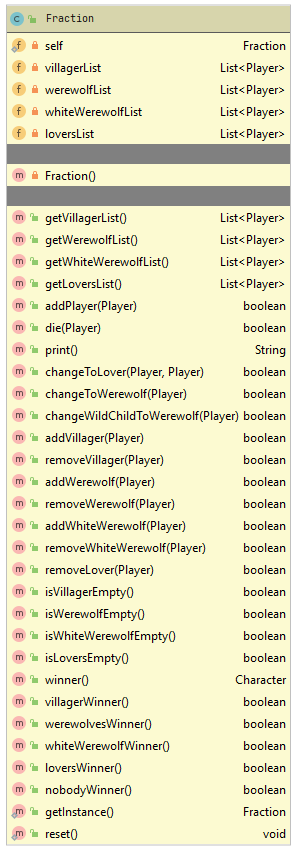
\includegraphics[width=0.45\textwidth]{architektur/fraction_uml.png}
	\caption{Fraction Übersicht}
	\label{figure:fraction_uebersicht}
\end{figure}

Wie in \autoref{figure:fraction_uebersicht} zu sehen besitzt die Klasse eine statische Klassenvariable, mit der Referenz auf das Singleton (\textit{self}). 
Weiterhin gibt es für die vier Fraktionen Dorfbewohner, Werwölfe, Weißer Werwolf und Liebespaar jeweils eine Liste mit den zugehörigen Spielern als Instanzvariable. 

\medskip
Für diese Listen gibt es jeweils eine \textit{get} Methode (z.B. \textit{getWerewolfList(): List<Player>}). 

\medskip
Es gibt sowohl eine Methode \textit{addPlayer(player: Player): boolean}, die einen übergebenen Spieler selbstständig zur richtigen Fraktion zuordnet, als auch für jede Fraktion eine eigene \textit{add} Methode (z.B. \textit{addWerewolf(player: Player): boolean}). Wenn jeweils keine Zuordnung zu einer Fraktion vorgenommen werden konnte, ist der Rückgabewert \textit{false}, im erfolgreichen Fall \textit{true}. Für jede Fraktion gibt es eine \textit{remove} Methode, um einen übergebenen Spieler aus der Fraktion zu entfernen. 

\medskip
Weiterhin gibt es für jede Fraktion eine Methode um zu prüfen, ob die jeweilige Fraktion keine Mitglieder enthält.

\medskip
Um zu testen, welche Fraktion gewonnen hat, gibt es zum Einen je Fraktion eine Methode, die prüft, ob die Fraktion gewonnen hat. Es gibt eine weitere Methode (\textit{winner(): Character}), die einen die Fraktion repräsentierenden Charakter zurückgibt, als Zeichen, welche Fraktion gewonnen hat. Ist hier der Rückgabewert \textit{null}, hat noch keiner gewonnen und das Spiel läuft noch. 

\medskip
Die Methode \textit{die(player: Player): boolean} entfernt einen übergebenen Spieler aus seiner Fraktion. 

\medskip
Mittels \textit{print(): String} lässt sich eine textuelle Repräsentation der Fraktionen generieren. 

\medskip
Mit der Methode \textit{changeToLover(player1: Player, player2: Player): boolean} lassen sich zwei Spieler zur Fratkion Liebespaar wechseln.
Die Methoden \textit{changetoWerewolf(player: Player): boolean} und \textit{changeWildChildToWerewolf(player: Player): boolean} wechseln einen beliebigen Spieler, bzw. das Wilde Kind, zur Fraktion der Werwölfe. 

\medskip
Um das Singleton zu erhalten, gibt es eine statische Methode \textit{getInstance(): Fraction}. 
Um das Singleton für eine neue Spielrunde zu reseten, gibt es die statische Methode \textit{reset(): void}. 

\subsection{Victim}

Das Package \textit{victim} enthält eine abstrakte Klasse \textit{Victim}, von der die einzelnen Opfer-Klassen erben. Außerdem befindet sich hier die Klasse \textit{Victims}, die die Opfer verwaltet und Zugriff auf sie gewährt. 

\medskip
\textit{Victims} hat je Opfer-Klasse eine Referenz auf dieses Opfer. 
Für jedes Opfer gibt es eine \textit{get} und eine \textit{set} Methode. 
Um abzufragen, ob es Nacht- oder Tagopfer gibt, gibt es die Methoden \textit{hasNightVictims(): boolean} bzw. \textit{hasLynchVictims(): boolean}. 
Abschließend gibt es eine Methode, um \textit{Victims} zu reseten (\textit{reset(): void}), sowie eine Methode \textit{print(): String}, um eine textuelle Repräsentation des Zustands von \textit{Victims} zu bekommen. 

\medskip
Die abstrakte Klasse \textit{Victim} speichert die Referenz auf einen Spieler, und die Todesursache als Text. 
Um diese abzufragen, existieren die Methoden \textit{getPlayer(): Player}, \textit{getDeathReason(): String} und \textit{isSet(): boolean}. Die letztgenannte Methode ist dazu da, um zu prüfen, ob das Opfer gesetzt wurde. Ansonsten ist der Rückgabewert bei \textit{getPlayer()} \textit{null}. 

\medskip
Jedes von \textit{Victim} abgeleitete Opfer hat zwei Konstruktoren, um das Objekt anzulegen und ein Attribut für die jeweilige Todesursache. Die eine Variante legt ein "leeres" Opfer an, die zweite eines mit Spieler und Todesursache. 
Einzig das Werwolf Opfer (\textit{VictimWerewolf}) hat noch weitere Methoden und Attribute. 
Hier gibt es noch Attribute, die speichern ob das Werwolf Opfer geheilt (\textit{healed}) oder infiziert (\textit{infected}) wurde. Dazu existieren Methoden diesen Zustand abzufragen, sowie um zu heilen, oder zu infizieren. 

\subsection{Trade}
\begin{figure}[H]
	\centering
	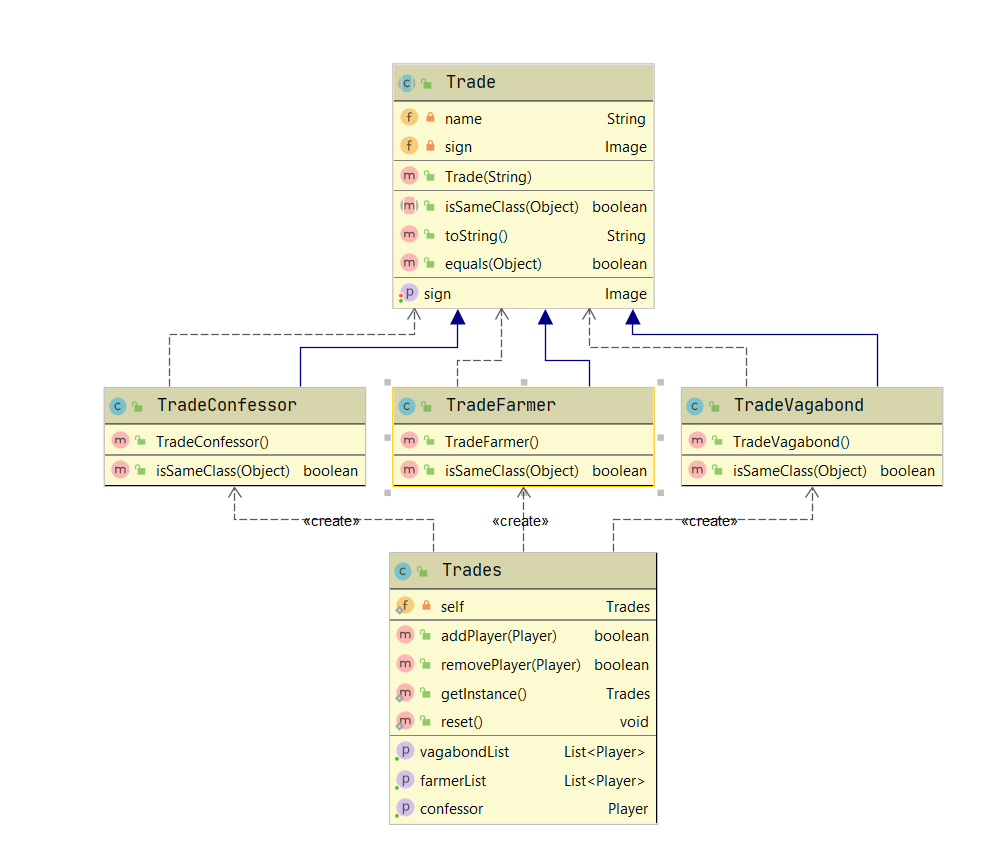
\includegraphics[width=\textwidth]{architektur/Trade_Uebersicht.png}
	\caption{Übersicht Trade (Package)}
	\label{figure:trade_uebersicht}
\end{figure}

Alle Berufe sind von der abstrakten Klasse \textit{Trade} abgeleitet, wie in \autoref{figure:trade_uebersicht} zu sehen ist. Dadurch ist für jeden Beruf eine einheitliche Ansprache gewährleistet und es können ohne weiteres neue Berufe implementiert werden.

\medskip
\textit{Trades} ist als Singleton implementiert, wo alle Informationen über die Spieler mit ihren Berufen gespeichert sind und somit im Spielverlauf auf bestimmte Berufe einzugehen, wenn sie eine bestimmtes Verhalten haben.
Die Methode \textit{reset()} setzt die Trades neu wenn ein neues Spiel gestartet wird.
\textit{addPlayer()} setzt die Spieler in die richtige Liste, welchen Beruf diese haben. Die Methode \textit{removePlayer()} wird aktiv, wenn ein Spieler im Spiel stirbt. Über die Methode \textit{getInstance()} kann man auf diezuvor genannten Methoden zugreifen.

\medskip
\textit{TradeConfessor}, \textit{TradeVagabond} und \textit{TradeFarmer} sind identisch aufgebaut, deshalb werden wir anhand der Klasse \textit{TradeFarmer} einmal erklären, wie die Methoden in den Klassen funktionieren.
In den jeweiligen Konstruktoren wird die Bezeichnung des Berufes gesetzt und auch sein Bild gesetzt, wo durch im Spiel ersichtlich ist, welcher Spieler welchen Beruf hat.
  
\section{View}

\begin{figure}[H]
	\centering
	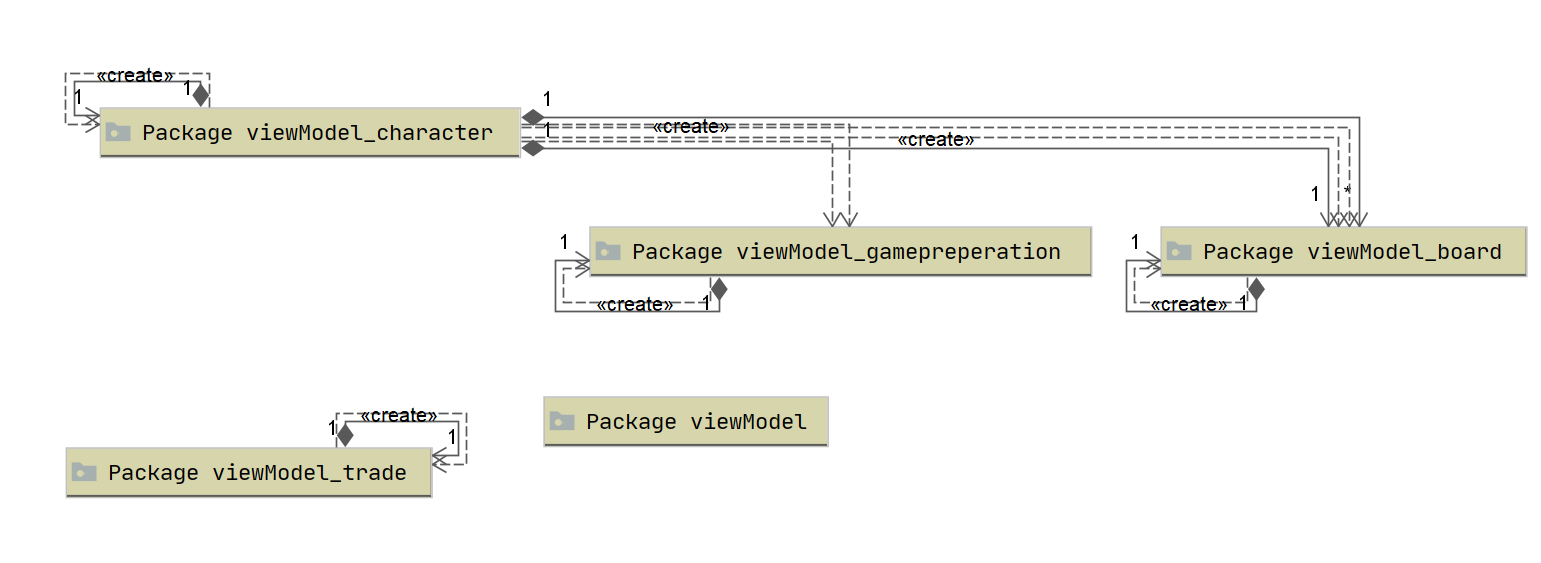
\includegraphics[width=\textwidth]{architektur/View_Packages_Uebersicht.png}
	\caption{Übersicht View}
	\label{figure:view_package_uebersicht}
\end{figure}

Die \autoref{figure:view_package_uebersicht} gibt einen Übersicht über die kompletten Packages der View, hierzu kommt noch der \textit{SceneManager}. 
In den folgenden Unterkapiteln wird genauer auf die Packages eingegangen. 

\subsection{ViewModel (Package)}

\begin{figure}[H]
	\centering
	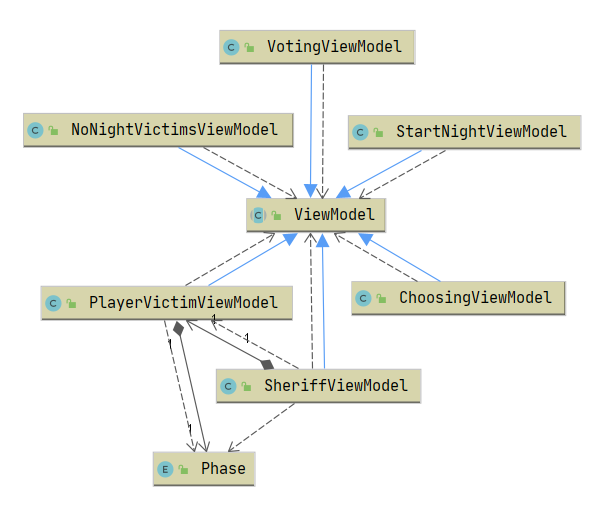
\includegraphics[width=\textwidth]{architektur/View_Uebersicht.png}
	\caption{Übersicht ViewModel (Package)}
	\label{figure:viewmodel(package)}
\end{figure}

Die \autoref{figure:viewmodel(package)} gibt eine grobe Übersicht über die View an. Die Hauptklasse, der View, ist die Klasse \textit{ViewModel}. Die Klasse \textit{VotingViewModel} ermöglicht es den Spielleiter bei einer Wahl zu unterstützen. Um Spieler auszuwählen ist die Klasse \textit{ChoosingViewModel} zuständig. Die Klasse \textit{StartNigthViewModel} wird verwendet für den ersten Start der Nacht, um die richtige nachfolgende Szene zu laden. Das \textit{PlayerVictimViewModel} kann bestimmte Phasen auslösen, wo noch ein weiteres Opfer ausgesucht werden muss oder eine Nachfolge bestimmt werden muss. 
Die Klasse \textit{SheriffViewModel} ist für die Wahl des Hauptmannes zuständig und wenn der Hauptmann stirbt wird, hierüber der Nachfolger bestimmt, welcher vom alten Hauptmann bestimmt wird. Die \textit{NoNightVictimsViewModel} Klasse springt zur nächsten richtigen Szene, die die Hauptmannwahl sein kann oder gleich schon die Lynchabstimmung.

\medskip
Bei der Klasse \textit{ChoosingViewModel} werden wir uns bestimmte Methoden anschauen, welche besonders wichtig sind für den Spielverlauf.
Die \textit{getStart()} Methode markiert für die jeweilige Szene das Liebespaar, welche sich nicht gegenseitig umbringen dürfen.
In der Methode \textit{choosing()} wird die richtige Methode von updateDisplay ausgewählt, für die beiden Szene, welche über das ViewModel angesprochen werden.
Die nextScene Methoden rufen in dem Fall die richtige nachfolgende Szene auf.

\medskip
Die Klasse \textit{VotingViewModel} wird die Abstimmung für das Lynchen am Tag auf gesetzt, welches in der Methode \textit{getStart()} passiert. Die Methoden \textit{nextSceneSheriff...()} sind bei gleichstand vorhandene Actionlistener, welche die Buttons abfragen, welchen der Hauptmann von ihnen umbringen möchte, aber nur wenn ein Hauptmann gewählt wurde. sonst wird in der Methode \textit{getStarted()} eine Stichwahl ausgeführt, mit den Spielern die ein gleichstand haben, außer einer hat mehr.
\textit{reset()} resetet die Comboboxen vom vorherigen Tag und auch die Labels.

\medskip
In der Klasse \textit{SheriffViewModel} wird die Logik für die Wahl des Hauptmannes programmiert. Wenn bei der Wahl ein gleichstand zustande kommt wird nochmals gewählt, wie bei dem \textit{VotingViewModel}, aber wenn es erneut zu einem Gleichstand kommt wird am nächsten Tag erneut gewählt. Diese Klasse hat ein paar extra Methoden und zwar wenn der Hauptmann stirbt, muss er seinen Nachfolger ernennen.

\medskip
Die Klassen \textit{StartNightViewModel} und \textit{NoNightVictimViewModel} sind in teilen identisch, sie unterscheiden sich nur in den aufrufen der nachfolgenden Szenen.

\medskip
Die letzte Klasse in dem Package \textit{PlayerVictimViewModel} behandelt die getöteten Spieler der Runde, damit die der Spielleiter ein Übersicht hat wer alles gestorben ist, um es den Mitspielern mitzuteilen und manche Rollen haben noch eine bestimmte Fähigkeit, wenn sie sterben, welche dann auch abgehandelt wird in der Szene.      

\subsection{ViewModel Board (Package)}

\begin{figure}[H]
	\centering
	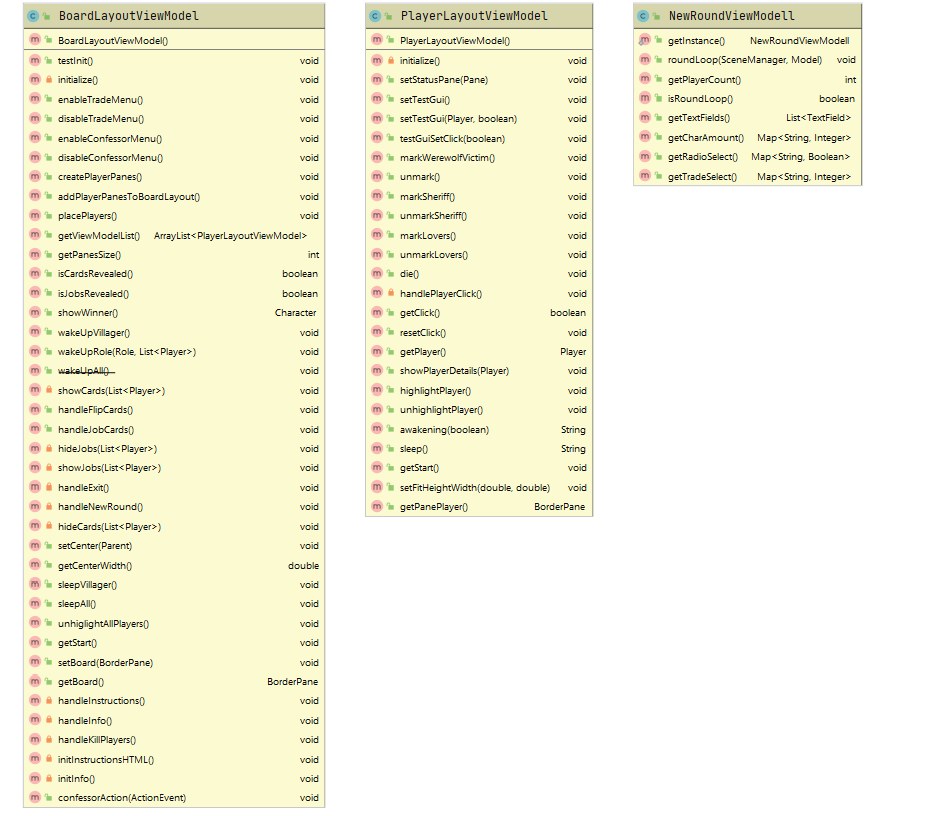
\includegraphics[width=\textwidth]{architektur/View_Board_Uebersicht.png}
	\caption{Übersicht ViewModel Board (Package)}
	\label{figure:viewmodelboard(package)}
\end{figure}

Die Klasse \emph{BoardLayoutViewModel} dient dazu das gesamte Spielfeld anzuzeigen. Auf diesem werden später alle Spieler platziert, sowie alle weiteren Informationen im Laufe des Spiels angezeigt. Dazu basiert das Spielfeld auf einer JavaFX-BorderPane. Die Klasse enthält einige Methoden um Nutzerinteraktionen z.B. über die Menüleiste zu erhalten. Außerdem bietet sie den anderen Programmteilen die Möglichkeit Szenen im Centerfield des BorderPanes anzeigen zu lassen. Weiterhin werden die in der Spielvorbereitung angelegten Spieler entsprechend ihrer Position auf dem Spielfeld platziert. Die maximale mögliche Größe der einzelnen Spielerkarten wird dabei von dieser Klasse errechnet und in den einzelnen Karten festgelegt um in der gegebenen Bildschirmauflösung alle Karten darstellen zu können.

\medskip
Die Klasse \emph{PlayerLayoutViewModel} dient dazu die einzelnen Karten der Spieler auf dem Spielfeld anzuzeigen. Dazu bietet sie Zugriff auf die Elemente der FXML-Datei und setzt hier entsprechend die benötigten CSS-Klassen. Außerdem beinhaltet die Klasse eine Möglichkeit auf Klicks zu reagieren und dabei die Spielerkarte entsprechend zu markieren. Zusätzlich bietet sie die Möglichkeit die Charakterkarte eines Spielers bei seinem Tod in Graustufen darzustellen und sein Statusfeld entsprechend einzufärben. Die Klasse enthält zusätzlich eine Möglichkeit die Größe der Spielerkarte festzulegen.

\medskip
Die Klasse \textit{NewRoundViewModel} wird verwendet wenn der Spielleiter eine Runde zu ende gespielt hat und eine neue Runde anfangen möchte, um das Programm nicht neu zu starten muss. Diese kann der Spielleiter auch während einer laufenden Runde. Es werden alle Information über die Auswahl der Runde gespeichert, welche er in den Szenen zur Gamepreparation anpassen kann.
  

\subsection{ViewModel Character (Package)}

\begin{figure}[H]
	\centering
	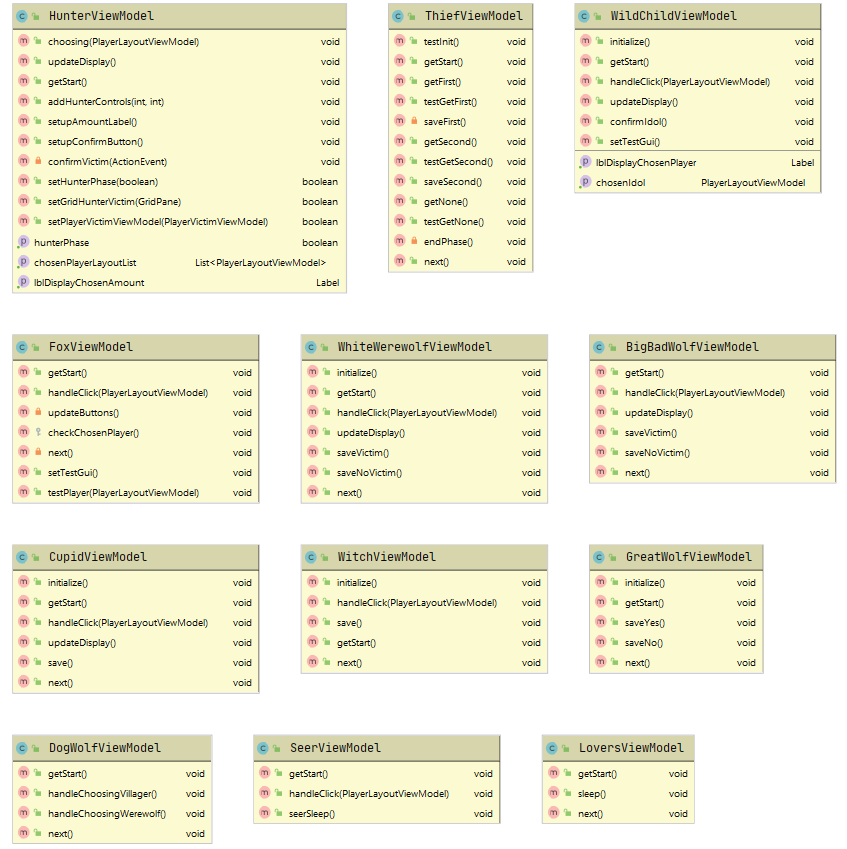
\includegraphics[width=\textwidth]{architektur/View_Char_Uebersicht.png}
	\caption{Übersicht ViewModel Character (Package)}
	\label{figure:viewmodelchar(package)}
\end{figure}

Es wird hier nur auf ein paar Klassen des Package, da die Klassen alle sehr ähnlich Aufgebaut sind.
Die Klassen \textit{SeerViewModel} und \textit{LoversViewModel} sind sehr identisch, sie unterscheiden sich nur in einer Methode, da die Seherin sich pro Nacht eine Karte anschauen kann.

\medskip
Das \textit{ThiefViewModel} merkt sich die Auswahl des Diebes vom Anfang der Spielrunde, um ihn der entsprechenden Fraktion zu zuordnen.

\medskip
Alle Klassen bis auf die \textit{LoversViewModel} haben eine Methode, welche sich um die Auswahl eines anderen Mitspieler kümmert, um die bestimmten Fähigkeiten der Rollen aus zu führen. 

\subsection{ViewModel Gamepreperation (Package)}

\begin{figure}[H]
	\centering
	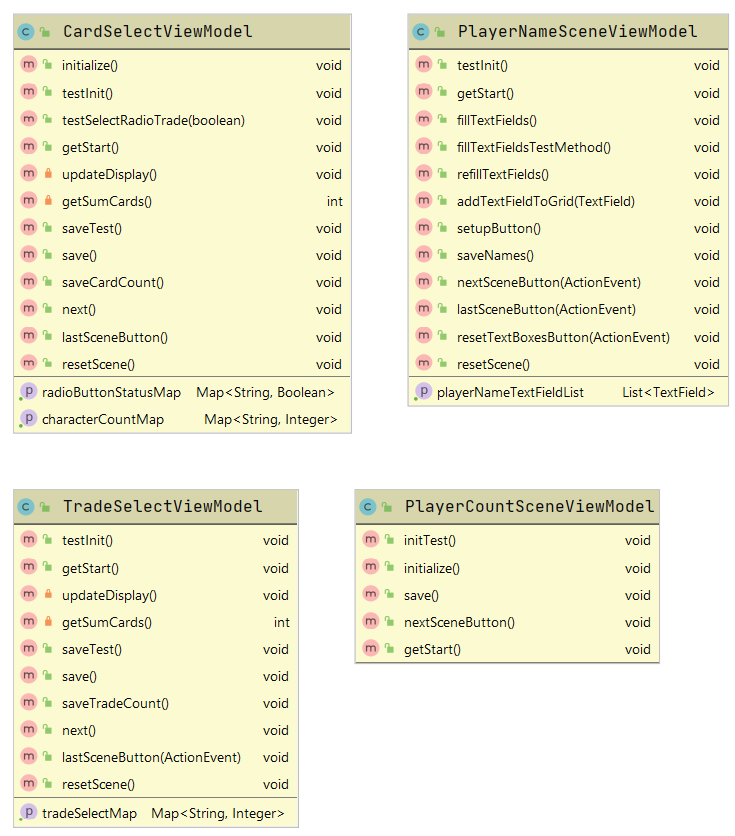
\includegraphics[width=\textwidth]{architektur/View_Game_Uebersicht.png}
	\caption{Übersicht ViewModel Gamepreperation (Package)}
	\label{figure:viewmodelgame(package)}
\end{figure}

Die Klassen in der \autoref{figure:viewmodelgame(package)} zusehen sind, dienen der Voreinstellung für eine Spielrunde getätigt, wenn eine neue Runde über den Loop gestartet wird, werden die Voreinstellungen der Runde zuvor übernommen. Alle Klassen haben die ähnliche Methoden, um die Auswahl zu speichern.
\subsection{ViewModel Trade (Package)}

\begin{figure}[H]
	\centering
	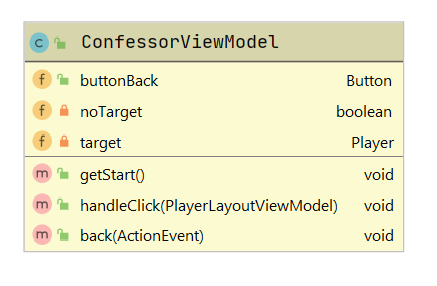
\includegraphics[width=0.6\textwidth]{architektur/View_Trade_Uebersicht.png}
	\caption{Übersicht ViewModel Trade (Package)}
	\label{figure:viewmodeltrade(package)}
\end{figure}

Die Klasse in dem Package behandelt die besondere Funktion des Beichtvaters, welche nur einmal verwendbar ist momentan.

\subsection{SceneManager}

Der \textit{SceneManager} ist die Hauptklasse um die Szenen zu initialisieren und zu laden. Die meisten FXML-Datein werden über die \textit{initFXML()} geladen. Manche Szenen werden über spezielle \textit{init...()} Methoden geladen, da die Szenen Informationen aus vorherigen Szenen benötigen. Die Szenen werden über die \textit{switchToScene()} Methode aufgerufen, über eine switch case wird zwischen den Szenen gewechselt. 

\section{Config}

Der Werwolf-Spielleiter erlaubt dem Benutzer verschiedene Werte der Software über eine JSON Config-Datei anzupassen. Als Beispiel dient hier der Standardwert an Mitspielern welcher beim Start automatisch selektiert wird. Die dazugehörige Config-Datei wird im Wurzelverzeichnis der Software eingelesen oder wenn sie noch nicht existiert, erstellt und mit Standardwerten gefüllt. Die dafür benötigten Klassen werden im Folgenden erläutert.

\subsection{ConfigLoader}

Die \textit{ConfigLoader} Klasse liest alle Konstanten aus der Klasse \textit{PublicGameConstants} aus und fügt diese der \textit{publicGameConstants} Liste hinzu. Mit der Methode \textit{initConfig} wird die Liste mit einer Liste verglichen die der \textit{JSONConfigLoader} aus einer Config-Datei eingelsen hat. Beim Start des Spiels wird an verschiedenen Stellen im Modell die \textit{getOrDefault} Methode aufgerufen. Diese liefert entweder ein Wert den der \textit{JSONConfigLoader} eingelesen hat oder einen Standardwert (Abbildung \ref{lst:configLoader01}).

\medskip
\begin{center}
	\begin{minipage}{0.95\textwidth}
		\lstinputlisting[firstnumber=80, firstline=80, lastline=96, caption=ConfigLoader getOrDefault Methode, label= lst:configLoader01]{../src/main/java/de/werwolf_spielleiter/config/ConfigLoader.java}
	\end{minipage}
\end{center}

\subsection{JSONConfigLoader}

Die \textit{JSONConfigLoader} Klasse wird von der \textit{ConfigLoader} Klasse verwendet um Config-Werte von einem vorgegebenen Pfad aus einer JSON Datei zu lesen. Existiert die Config-Datei unter dem Pfad, dann werden alle ausgelesene Werte dem \textit{ConfigLoader} über den Aufruf der Methode \textit{readConfigFromJSON} übergeben. Existiert die Config-Datei nicht, dann wird eine neue Config-Datei erstellt, welche die Standardwert der \textit{PublicGameConstants} Klasse enthält.

\section{Anspruchsvolle Stellen der Implementierung}

Ein besonders zu Beginn schwieriges Thema war die korrekte Erstellung der FXML-Dateien. Zunächst wurden viele FXML-Dateien separat  angelegt. Durch die vielen Einstellungsmöglichkeiten war es nicht immer ganz einfach, später diverse Einstellungen in csv-Dateien auszulagern. 

\medskip
Ein weiteres Thema war die Initialisierung der FXML-Dateien. Wir haben teilweise einige Anläufe gebraucht, diese korrekt zu initialisieren. Besonders wenn in den Szenen Daten aus dem Spielverlauf benötigt werden, die zu Beginn beim Programmaufruf noch nicht vorhanden sind. Dort wurde aber nach einiger Zeit eine passable Lösung gefunden. 

\medskip
Ein anspruchsvoller Punkt war das Einrichten der Build-Pipeline für JavaFx, da die normale Pipeline um weitere Befehle ergänzt werden musste.

\chapter{Testkonzept}
In diesem Kapitel wird das umgesetzte Testkonzept des Softwareprojekts beschrieben. Dieses besteht dabei aus automatisierten Tests mittels JUnit, welche in \autoref{sec:automatisierteTests} näher beschrieben werden, sowie aus manuellen Tests für das User Interface. Letztere werden in \autoref{sec:manuelleTests} beschrieben.

\section{Automatisierte Tests}
\label{sec:automatisierteTests}
Zum Testen des \emph{Models} werden automatisierte Tests mittels JUnit verwendet. Dabei wird eine Testabdeckung von 100\% angestrebt, welche auch nahezu erreicht wird. Das \emph{ViewModel} wird nur teilweise automatisiert getestet, weshalb hier eine niedrigere Testabdeckung erreicht wird. Die nicht mit Tests abgedeckten Teile des \emph{ViewModels} sind überwiegend \emph{GUI}-Bestandteile und werden, wie in \autoref{sec:manuelleTests} beschrieben getestet.
\section{Manuelle Tests}
\label{sec:manuelleTests}
Um auch die Teile der Software zu testen, die nicht durch die in \autoref{sec:automatisierteTests} beschriebenen automatisierten Tests abgedeckt werden, wurden eine Reihe von manuellen Testfällen entwickelt. Diese sind insgesamt in unserem Projektwiki zu finden und werden hier der Übersicht halber nur ausschnittsweise gezeigt.
	\subsection{Tests zur Spielvorbereitung}
		\subsubsection{Spieleranzahl}
			\begin{packed_itemize}
				\item[\(\square\)] Karten umdrehen und Berufe anzeigen hat keine Auswirkungen
				\item[\(\square\)] Neues Spiel starten hat keine Auswirkungen
			\end{packed_itemize}
		\subsubsection{Spielernamen}
			\begin{packed_itemize}
				\item[\(\square\)] Karten umdrehen und Berufe anzeigen hat keine Auswirkungen
				\item[\(\square\)] Neues Spiel starten hat keine Auswirkungen
			\end{packed_itemize}
		\subsubsection{Kartenauswahl}
			\begin{packed_itemize}
				\item[\(\square\)] Karten umdrehen und Berufe anzeigen hat keine Auswirkungen
				\item[\(\square\)] Neues Spiel starten hat keine Auswirkungen
			\end{packed_itemize}
		\subsubsection{Kartenverteilung (Start Game)}
			\begin{packed_itemize}
				\item[\(\square\)] Es wurden so viele Spieler platziert, wie festgelegt.
				\item[\(\square\)] Die eingegebenen Namen der Spieler werden angezeigt.
				\item[\(\square\)] Die Charakterkarten sind anhand der ausgesuchten Menge verteilt. (Mit Dieb sind zwei Karten nicht an die Spieler verteilt worden.)
				\item[\(\square\)] mit Berufe: die Berufsplättchen wurden entsprechend der eingegebenen Anzahl verteilt.
				\item[\(\square\)] ohne Berufe: die Charakterkarten lassen sich umdrehen.
				\item[\(\square\)] mit Berufe: die Charakterkarten lassen sich umdrehen
				\item[\(\square\)] mit Berufe: die Berufsplättchen lassen sich anzeigen.
			\end{packed_itemize}
\include{sections/05_dod}
\chapter{Branching Modell}

Beim Branching Modell wurde ein Modell ähnlich dem Dezentralen Branching Modell verwendet. Im Zentrum steht der Master Branch welche den derzeitigen Stand aller fertig entwickelten Features enthält. Um das Zentrum herum gibt es Feature Branches in denen aktiv Features entwickelt und getestet werden. Untereinander tauschen diese Feature Branches auch ihre Änderungen aus. Ist eine Feature Branch fertig getestet und überprüft, wird sie in den Master Branch gemerged und geschlossen.

\begin{figure}[H]
	\centering
	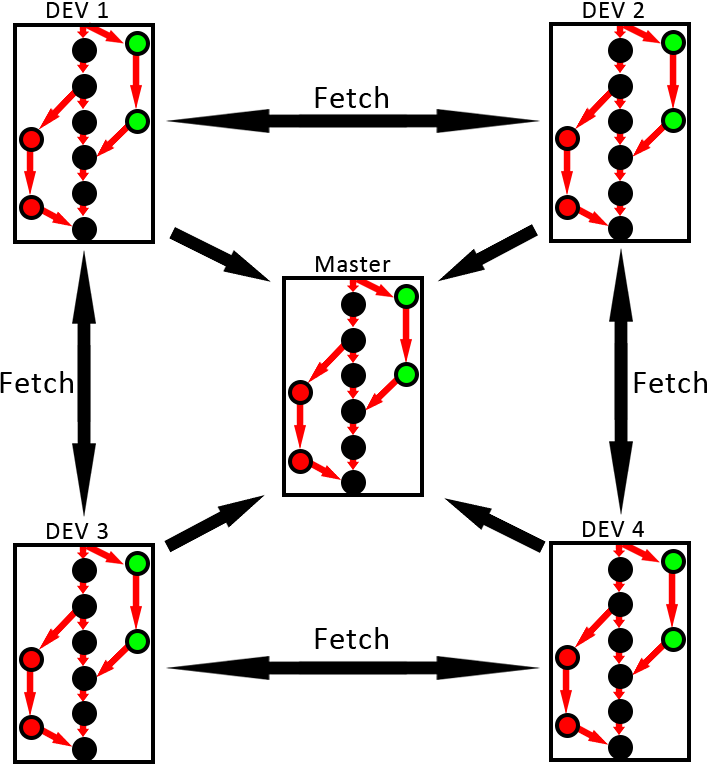
\includegraphics[width=0.7\textwidth]{branch/center_repo.png}
	\caption{Projekt Branching Modell}
	\label{figure:diagram_branching_model}
\end{figure}
\chapter{Test-, Buildautomatisierung, CI}

Das Projekt Werwolf-Spielleiter wird in einer CI-Pipeline bei jedem Push auf eine Branch automatisch getestet und gebaut. Hierfür verwendet werden Runners der Technischen Hochschule Lübeck und GitLab als Platfform für die Versionskontrollsystem. Die Software selber wird, wie in Abbildung \ref{lst:ymlConfig01} dargestellt, in einem Maven Docker Container getestet und gebaut. Die Konfiguration der CI-Pipeline erfolgt über eine GitLab CI YML Datei. Im Folgenden wird diese genauer erläutert.

\medskip
\begin{center}
	\begin{minipage}{0.7\textwidth}
		\lstinputlisting[firstnumber=1, firstline=1, lastline=1, caption=Projekt CI Docker-Konfiguration, label= lst:ymlConfig01]{../.gitlab-ci.yml}
	\end{minipage}
\end{center}

\section{Testautomatisierung}

Bevor das Projekt gebaut wird, werden immer erst alle Unit-Tests ausgeführt. Schlägt ein Test fehl wird die Pipeline abgebrochen bzw. der Build-Prozess erfolgt nicht. Die Unit-Tests werden von dem Build-Management-Tool Maven aufgerufen und Headless getestet, siehe Abbildung \ref{lst:ymlConfig02} Zeile 10. Da der Werwolf-Spielleiter das JavaFX Framework verwendet, wird dies benötigt. Die Unit-Tests testen nicht nur das Modell, sondern auch andere Teile der Software, wie zum Beispiel ob die richtige Anzahl an Textfeldern angezeigt wird.

\medskip
\begin{center}
	\begin{minipage}{0.7\textwidth}
		\lstinputlisting[firstnumber=7, firstline=7, lastline=10, caption=Projekt CI Test-Konfiguration, label= lst:ymlConfig02]{../.gitlab-ci.yml}
	\end{minipage}
\end{center}

Des Weiteren wird für die Headless Tests das Modul Monocle von TestFX verwendet. Dieses emuliert ein Software Display auf dem die JavaFX Anwendung angezeigt werden kann. Das Modul wird durch Maven automatisch nachgeladen (Abbildung \ref{lst:pomConfig01}) und in der GitLab CI YML Datei im Maven Test Befehl eingebunden (Abbildung \ref{lst:ymlConfig02} Zeile 10).

\medskip
\begin{center}
	\begin{minipage}{0.7\textwidth}
		\lstinputlisting[firstnumber=244, firstline=244, lastline=249, caption=Maven POM CI Test-Konfiguration, label= lst:pomConfig01]{../pom.xml}
	\end{minipage}
\end{center}

\section{Buildautomatisierung}

Wenn alle Test positiv waren erfolgt der Build-Prozess. Dafür werden die Befehle \textit{clean} und \textit{package} von Maven verwendet (Abbildung \ref{lst:ymlConfig03}). Durch \textit{clean} werden vorherige Build Artefakte und temporäre Dateien gelöscht. Mit dem Zusatz \textit{Dmaven.test.skip} werden die Tests übersprungen die normalerweise mit dem Befehl \textit{package} mit ausgeführt werden. Dies ist aufgrund dessen, da die Test in einer separaten Sektion vorher schon ausgeführt wurden. Außerdem ist hier ein Pfad angegeben, wo sich die gebauten Artefakte nach dem Build-Prozess befinden, damit diese automatisch von GitLab aufgegriffen und zum Download angeboten werden können.

\medskip
\begin{center}
	\begin{minipage}{0.7\textwidth}
		\lstinputlisting[firstnumber=12, firstline=12, lastline=18, caption=Projekt CI Build-Konfiguration, label= lst:ymlConfig03]{../.gitlab-ci.yml}
	\end{minipage}
\end{center}

Gebaut werden die JAR-Dateien für die Plattformen Windows, Linux und Mac. Hierfür wurden die JavaFX Abhängigkeiten von allen Plattformen in die Maven POM des Projekts eingebunden. Außerdem wird das Maven Plugin Shade verwendet um eine Fat JAR zu erzeugen, damit beim Start der Anwendung keine Abhängigkeiten von JavaFX nachgeladen werden müssen.

\medskip
\begin{center}
	\begin{minipage}{0.8\textwidth}
		\lstinputlisting[firstnumber=238, firstline=238, lastline=242, caption=Maven POM Build-Konfiguration, label= lst:pomConfig02]{../pom.xml}
	\end{minipage}
\end{center}
\chapter{Schätzung}

Die Issues wurden gemeinsam in den Schätz- und Sprintplannungs Meetings geschätzt. Dabei wurden die Sprints folgendermaßen geschätzt:
\begin{itemize}
\item Sprint 1: 65 Storypoints
\item Sprint 2: 48,5 Storypoints
\item Sprint 3: 49 Storypoints
\item Sprint 4: 59 Storypoints
\item Sprint 5: 48 Storypoints
\end{itemize}
\chapter{Burndown-Charts}

Die Burndown-Charts zeigen nur vollständigen Issues an.

\section{Sprint 1}

\begin{figure}[H]
	\centering
	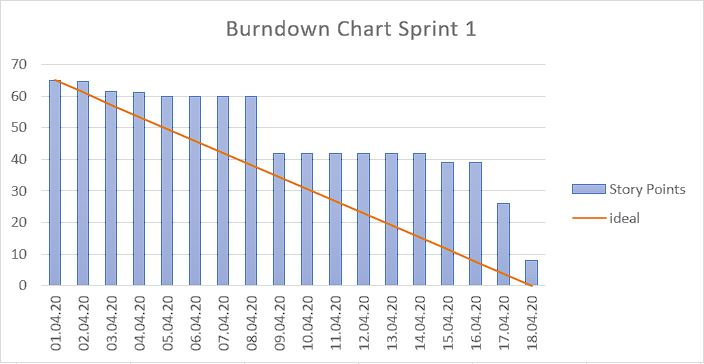
\includegraphics[width=\textwidth]{burndown/sprint1.jpg}
	\caption{Burndowndiagramm Sprint 1}
	\label{figure:burndown_sprint1}
\end{figure}

Im ersten Sprint, vom 01.04.2020 bis zum 18.04.2020, haben wir 65 Storypoints für 20 Issues geschätzt. Am Ende des Sprint ist ein Issue mit 8 Storypoints noch nicht vollständig abgeschlossen gewesen.
\begin{itemize}
\item Scrum Master: Henrik Möhlmann
\item Product Owner: Janik Dohrmann
\end{itemize}

\newpage
\section{Sprint 2}

\begin{figure}[H]
	\centering
	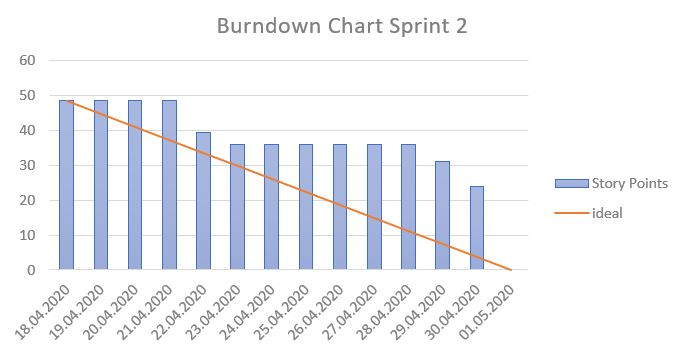
\includegraphics[width=\textwidth]{burndown/sprint2.jpg}
	\caption{Burndowndiagramm Sprint 2}
	\label{figure:burndown_sprint2}
\end{figure}

Im zweiten Sprint, vom 18.04.2020 bis zum 01.05.2020, haben wir 48,5 Storypoints für 11 Issues geschätzt. Am Ende des Sprints waren alle Issues abgearbeitet.
\begin{itemize}
\item Scrum Master: Eric De Ron
\item Product Owner: Florian Müller
\end{itemize}

\newpage
\section{Sprint 3}

\begin{figure}[H]
	\centering
	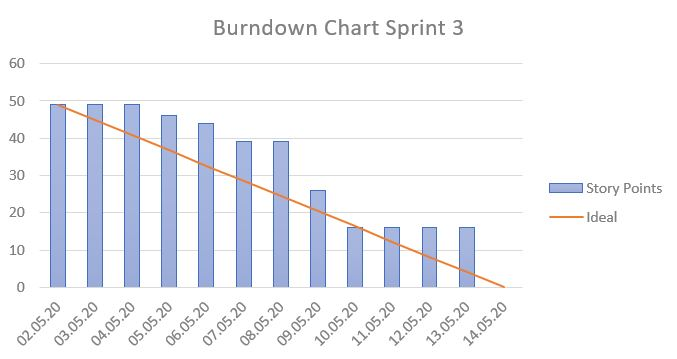
\includegraphics[width=\textwidth]{burndown/sprint3.jpg}
	\caption{Burndowndiagramm Sprint 3}
	\label{figure:burndown_sprint3}
\end{figure}

Im dritten Sprint, vom 02.05.2020 bis zum 14.05.2020, haben wir 49 Storypoints für 10 Issues geschätzt. Am Ende des Sprints waren alle Issues abgearbeitet.
\begin{itemize}
\item Scrum Master: Matthias Hinrichs
\item Product Owner: Alonso Essenwanger
\end{itemize}

\newpage
\section{Sprint 4}

\begin{figure}[H]
	\centering
	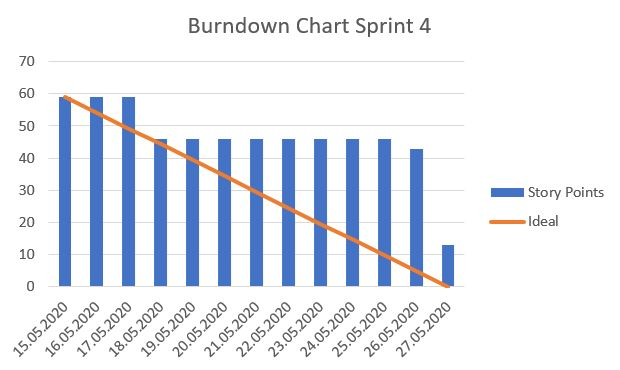
\includegraphics[width=\textwidth]{burndown/sprint4.jpg}
	\caption{Burndowndiagramm Sprint 4}
	\label{figure:burndown_sprint4}
\end{figure}

Im vierten Sprint, vom 15.05.2020 bis zum 27.05.2020, haben wir 59 Storypoints für 9 Issues geschätzt. Am Ende des Sprints ist ein Issue mit 13 Storypoints noch nicht vollständig übergeblieben.
\begin{itemize}
\item Scrum Master: Janik Dohrmann
\item Product Owner: Eric De Ron
\end{itemize}

\newpage
\section{Sprint 5}

\begin{figure}[H]
	\centering
	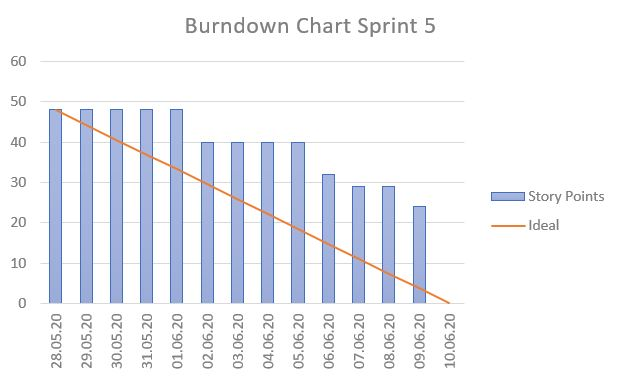
\includegraphics[width=\textwidth]{burndown/sprint5.jpg}
	\caption{Burndowndiagramm Sprint 5}
	\label{figure:burndown_sprint5}
\end{figure}

Im fünften Sprint, vom 28.05.2020 bis zum 10.06.2020, haben wir 48 Storypoints für 7 Issues geschätzt. Am Ende des Sprints waren alle Issues abgearbeitet.
\begin{itemize}
\item Scrum Master: Florian Müller
\item Product Owner: Henrik Möhlmann
\end{itemize}

\chapter{Velocity des Teams}

Pro Sprint haben wir durchschnittlich 53,9 Storypoints geschätzt. Dabei haben wir durchschnittlich 11,4 Issues pro Sprint umgesetzt.
\include{sections/11_reflektion}
\chapter{Protokoll der Tätigkeiten der Teammitglieder}

\section{Tätigkeiten Eric De Ron}

\begin{tabularx}{\textwidth}{|l|p{4.5cm}|l|X|}
	\hline                                             % Gitterlinie oberhalb
	\textbf{\#}  &    \textbf{Bezeichnung}  &    \textbf{Typ}  & \textbf{Beschreibung}	 \\ 
	\hline \hline 
	\endhead      
	
	5 \label{iss:5}	&	Spieleranzahl soll eingegeben werden können &	Feature	&	Benutzer kann über einen Slider die Spieleranzahl anpassen  \\ \hline
	6 \label{iss:6}	&	Spielernamen sollen eingegeben werden können    &	Feature	&	Benutzer kann über Textfelder Namen der Mitspieler eingeben  \\ \hline
	8 \label{iss:8}	&	Die Opfer der Nacht sollen angezeigt werden &	Feature	&	Ein Element der View welches die Opfer der Nacht variabel anzeigt  \\ \hline
	18 \label{iss:18}	&	Gitignore erstellen &	Feature	&	Eine Git-Datei welche Intellij, Eclipse und NetBeansfiles Config-Dateien ausschließt  \\ \hline
	22 \label{iss:22}	&	Card select combobox crash  &	Bug	&	Die Comboboxen in der Card Select Szene wurden mit null initialisiert und erzeugten eine InvocationTargetException  \\ \hline
	23 \label{iss:23}	&	Konstanten in Konfigurationsdatei auslagern &	Feature	&	Benutzer kann Standardwerte der Software über eine JSON-Config-Datei anpassen, außerdem wurden alle Konstanten der Software ausgelagert  \\ \hline
	28 \label{iss:28}	&	Lynch Abstimmung Werwolf Auswahl bleibt bestehen	&	Bug	&	Ausgewählte Lynch Opfer waren auch in der Werwolf Opfer Anzeige ausgewählt  \\ \hline
	31 \label{iss:31}	&	Szenen Nummerierung / Bezeichnung in enum Klasse auslagern	&	Feature	&	Die Szenen Nummerierung des SceneManager wurden als Enum in eine separate Klasse ausgelagert  \\ \hline
	37 \label{iss:37}	&	Jäger einfügen	&	Feature	&	Implementieren des Jägers als Charakter mit eigender .fxml Datei. Hinzufügen eigender Szene in der Opfer Anzeige. Hinzufügen der Kurzanleitung.  \\ \hline
	46 \label{iss:46}	&	Zurück Button	&	Feature	&	In den Gamepreperation Szenen wird eine zurück Button angezeigt, welcher das zurück navigieren zu vorherigen Szenen erlaubt  \\ \hline
	59 \label{iss:59-2}	&	GUI Testfälle	&	Feature	&	GUI Testfälle ergänzt  \\ \hline
	69 \label{iss:69}	&	Wildes Kind einfügen    &	Feature	&	Implementieren des Wilden Kindes als Charakter mit eigender .fxml Datei. Hinzufügen eigender Szene in der ersten Nacht. Hinzufügen der Kurzanleitung.  \\ \hline
\caption{Tätigkeiten Eric De Ron}\label{tbl:eric}
\end{tabularx}

\newpage
\section{Tätigkeiten Janik Dohrmann}

\begin{tabularx}{\textwidth}{|l|p{4.5cm}|l|X|}
	\hline                                              % Gitterlinie oberhalb
	\textbf{\#}  &    \textbf{Bezeichnung}  &    \textbf{Typ}  & \textbf{Beschreibung}	 \\ 
	\hline \hline   
	\endhead
	
	2 \label{iss:2}	&	Dorfbewohner ins Spiel einfügen	&	Feature	&	Einfügen der Dorfbewohner ins Spiel  \\ \hline
	4 \label{iss:4}	&	Anzeigen Sieg einer Funktion	&	Feature	&	Implementieren der Anzeige für den Sieg einer Spielfunktion entsprechend der Regeln  \\ \hline
	10 \label{iss:10}	&	DoD erstellen	&	Feature	&	Erstellen der DoD in der Readme Datei im Repository  \\ \hline
	11 \label{iss:11}	&	Java Projekt erstellen	&	Feature	&	Erstellen des Java Projekts mit Java 13 und Maven  \\ \hline
	12 \label{iss:12}	&	CI Pipeline	&	Feature	&	Einrichten einer CI Pipeline für den Maven Test- und Buildprozess  \\ \hline
	30 \label{iss:30}	&	Package-Ordner Struktur ändern	&	Feature	&	Anpassen der Package/Order Struktur  an Aufgabenbereiche der Software\\ \hline
	39 \label{iss:39}	&	Seherin einfügen	&	Feature	&	Implementieren der Seherin als Charakter mit eigender .fxml Datei  \\ \hline
	50 \label{iss:50}	&	Maven package in CI Pipeline einfügen	&	Feature	&	In die CI Pipeline den Maven Befehl package einfügen  \\ \hline
	59 \label{iss:59-1}	&	GUI Testfälle	&	Feature	&	GUI Testfälle ergänzt  \\ \hline
	61 \label{iss:61}	&	Wenn alle Karten aufgedeckt sind wird durch Seherin ausgewählte Karte zugedeckt	&	Bug	&	Wenn alle Karten aufgedeckt sind wird durch Seherin ausgewählte Karte zugedeckt beim Einschlafen der Seherin zugedeckt \\ \hline
	63 \label{iss:63}	&	Vagabund einfügen	&	Feature	&	Implementieren des Vagabunden mit den Grundstrukturen für die Berufe und einer .fxml Datei für die Berufsauswahl   \\ \hline
	65 \label{iss:65}	&	Beichtvater einfügen	&	Feature	&	Implementieren des Beichtvaters mit einer .fxml Datei und einem Menüpunkt für die Tagaktionen der Berufe  \\ \hline
	71 \label{iss:71}	&	Anleitung zum Berufe programmieren schreiben	&	Feature	&	Eine Anleitung zum implementieren der Berufe im Wiki schreiben  \\ \hline
\caption{Tätigkeiten Janik Dohrmann}\label{tbl:janik}
\end{tabularx}

\newpage
\section{Tätigkeiten Alonso Essenwanger}

\begin{tabularx}{\textwidth}{|l|p{4.5cm}|l|X|}
	\hline                                              % Gitterlinie oberhalb
	\textbf{\#}  &    \textbf{Bezeichnung}  &    \textbf{Typ}  & \textbf{Beschreibung}	 \\ 
	\hline \hline 
	\endhead    
	
	1 \label{iss:1}	&	Werwölfe: Aufwachen	&	Feature	&	Implementiert die Option damit die Werwölfe aufwachen und sie farbig markiert werden  \\ \hline
	17 \label{iss:17}	&	Werwölfe: Einschlafen &	Feature	&	Implementiert die Option damit die Werwölfe einschlafen, die Markierung entfernt wird und es wird ein Text zum einschlafen der Werwölfe angezeigt  \\ \hline
	34 \label{iss:34}	&	Menüeintrag Spielanleitung/Infobox	&	Feature	&	Ein Menü Hilfe wurde erstellt mit der Spielanleitung und Info   \\ \hline
	49 \label{iss:49}	&	Farbiger Spielerstatus einführen 	&	Feature	&	Die Spieler besitzen ein farbiger Status. Die Karten werden zur Mitte des Spielfeldes angeordnet. Wenn ein Spieler stirbt wird die Karte grau angezeigt  \\ \hline
	55 \label{iss:55}	&	Hinweistext bei der Hexe	 &	Feature	&	Ein Hinweistext wird bei der Hexe angezeigt nur wenn sie noch töten darf  \\ \hline
	63 \label{iss:63-1}	&	Vagabund einfügen	&	Feature	&	Ein Menü für die Jobs wurde implementiert damit die Jobs angezeigt werden.  \\ \hline
	72 \label{iss:72}	&	Planung Usability Test	&	Feature	&	Usability Test mit LaTeX  \\ \hline
\caption{Tätigkeiten Alonso Essenwanger}\label{tbl:alonso}
\end{tabularx}

\newpage
\section{Tätigkeiten Matthias Hinrichs}

\begin{tabularx}{\textwidth}{|l|p{4.5cm}|l|X|}
	\hline                                              % Gitterlinie oberhalb
	\textbf{\#}  		& \textbf{Bezeichnung}				& \textbf{Typ}	& \textbf{Beschreibung}\\ \hline \hline  
	\endhead    	
	9 \label{iss:9}		& Spieler auf Spielfeld anzeigen	& Feature		& Für alle Spieler wird eine Karte auf dem Spielfeld angezeigt\\ \hline
	15 \label{iss:15}	& Karten umdrehen					& Feature		& Alle Spielerkarten können umgedreht werden\\ \hline
	29 \label{iss:29}	& CSS-Styles						& Feature		& Alle Stylings im Programm sind mit CSS umgesetzt\\ \hline
	32 \label{iss:32}	& FXML-Dateien umbauen				& Feature		& Alle FXML-Dateien sind so gebaut, dass sie möglichst kompakt sind, vertikal und horizontal zentriert werden und beim resizen des Programms nicht die Größe ändern\\ \hline
	33 \label{iss:33}	& Menüeintrag Beenden				& Feature		& Es gibt ein Menü mit einem Eintrag Beenden um das Programm zu beenden\\ \hline
	35 \label{iss:35}	& Menüeintrag Karten umdrehen		& Feature		& Der Menüeintrag um die Karten umzudrehen wird zu einem zusammengefasst\\ \hline
	41 \label{iss:41}	& Anzeigereihenfolge der Szenen		& Feature		& Das Boardlayout wird als erstes geladen und alle weiteren Szenen im Centerfield dargestellt\\ \hline
	51 \label{iss:51}	& Default Buttons					& Feature		& Alle weiterführenden Buttons werden als Default Buttons deklariert, damit sie mit Enter ausgelöst werden können\\ \hline
	52 \label{iss:52}	& Auflösungsoptimierung				& Feature		& Das Spiel ist für Full HD(1920x1080) und HD(1366x768) Bildschirme optimiert\\ \hline
	58 \label{iss:58}	& Markieren mit Rahmen				& Feature		& Spieler, die ausgewählt wurden, werden mit einem farbigen Rahmen markiert\\ \hline
	70 \label{iss:70}	& Fuchs einfügen					& Feature		& Es gibt den Charakter Fuchs entsprechend der Spielregeln\\ \hline
	73 \label{iss:73}	& Überlagernde Eingabefelder		& Bug			& Bei der Namenseingabe werden Eingabefelder überlagert\\ \hline
	74 \label{iss:74}	& Szenen zu groß					& Bug			& Bei verschiedenen Szenen kann es vorkommen, dass diese im Centerfield zu groß ist und den unteren Container der Spielerkarten aus dem Bild schiebt\\ \hline
\caption{Tätigkeiten Matthias Hinrichs}\label{tbl:matthias}
\end{tabularx}

\newpage
\section{Tätigkeiten Henrik Möhlmann}

\begin{tabularx}{\textwidth}{|l|p{4.5cm}|l|X|}
	\hline                                              % Gitterlinie oberhalb
	\textbf{\#}  &    \textbf{Bezeichnung}  &    \textbf{Typ}  & \textbf{Beschreibung}	 \\ 
	\hline \hline      
	\endhead
	
	7 \label{iss:7}	&	Kartenauswahl	&	Feature	&	Auswahl der Charakterkarten zu Spielbeginn  \\ \hline
	14 \label{iss:14}	&	Anzeige Lynch Opfer	&	Feature	&	Die Opfer der Lynch Abstimmung in der Mitte anzeigen und sterben lassen  \\ \hline
	19 \label{iss:19}	&	Spiel starten	&	Feature	&	Spiel initialisieren, Karten verteilen und mit erster Nacht beginnen; Backend initial programmieren  \\ \hline
	20 \label{iss:20}	&	Bilder Werwolf / Dorfbewohner	&	Feature	&	Bilder für Vorder- und Rückseite von Dorfbewohner und Werwolf einfügen  \\ \hline
	21 \label{iss:21}	&	Bug card select	&	Bug	&	Exceptions bei Klick auf \glqq weiter\grqq{} beheben  \\ \hline
	36 \label{iss:36}	&	Hexe einfügen (+ Anleitung Charakter Programmieren)	&	Feature	&	Hexe im Backend einfügen. Hexe im Frontend einfügen (inkl. eigener Scene). Anleitung zum Charakter programmieren schreiben.   \\ \hline
	38 \label{iss:38}	&	Amor einfügen	&	Feature	&	Amor und Liebespaar im Backend einfügen. Amor und Liebespaar im Frontend einfügen (jeweils inkl. eigener Scene).   \\ \hline
	40 \label{iss:40}	&	Kleines Mädchen einfügen	&	Feature	&	Kleines Mädchen im Backend einfügen. Kleines Mädchen im Frontend einfügen.   \\ \hline
	45 \label{iss:45}	&	Bug Spiel mit nur einer Fraktion	&	Bug	&	Wenn nur Charaktere einer Fraktion ausgewählt werden, das Spiel nicht starten, sondern gleich Gewonnen anzeigen.   \\ \hline
	47 \label{iss:47}	&	Highilight von Werwolfphase bleibt bei Lynch	&	Bug	&	Wenn die Werwölfe uneinig sind, die Markierungen zurücksetzen.   \\ \hline
	54 \label{iss:54}	&	Dieb einfügen	&	Feature	&	Dieb im Backend einfügen (inkl. Charakterwechsel). Dieb im Frontend einfügen (inkl. eigener Scene).   \\ \hline
	57 \label{iss:57}	&	Bug keiner kann gewinnen	&	Bug	&	Die Berechnung des Gewinns einer Fraktion anpassen, sodass der Gewinn zum richtigen Zeitpunkt angezeigt wird.   \\ \hline
	59 \label{iss:59}	&	GUI Testfälle	&	Feature	&	Initialen Satz GUI Testfälle erstellt  \\ \hline
	64 \label{iss:64}	&	Weißer Werwolf einfügen	&	Feature	&	Weißer Werwolf im Backend einfügen. Weißer Werwolf im Frontend einfügen (inkl. eigener Scene).   \\ \hline
	66 \label{iss:66}	&	Urwolf einfügen	&	Feature	&	Urwolf im Backend einfügen. Urwolf im Frontend einfügen (inkl. eigener Scene).   \\ \hline
	67 \label{iss:67}	&	Großer, böser Wolf einfügen	&	Feature	&	Großer, böser Wolf im Backend einfügen. Großer, böser Wolf im Frontend einfügen (inkl. eigener Scene).   \\ \hline
	68 \label{iss:68}	&	Wolfshund einfügen	&	Feature	&	Wolfshund im Backend einfügen. Wolfshund im Frontend einfügen. Einige GUI Tests durch JUnit Tests ersetzt.   \\ \hline
\caption{Tätigkeiten Henrik Möhlmann}\label{tbl:henrik}
\end{tabularx}

\newpage
\section{Tätigkeiten Florian Müller}

\begin{tabularx}{\textwidth}{|l|p{4.5cm}|l|X|}
	\hline                                              % Gitterlinie oberhalb
	\textbf{\#}  &    \textbf{Bezeichnung}  &    \textbf{Typ}  & \textbf{Beschreibung}	 \\ 
	\hline \hline      
	\endhead
	
	3 \label{iss:3}	&	Lynch Abstimmung: Spieler auswählen	&	Feature	&	Auswahl der Spieler für die Lynch Abstimmung ins Frontend und in das Backend (inkl. eigene Szene). \\ \hline
	13 \label{iss:13}	&	Lynch Abstimmung: Über Spieler abstimmen	&	Feature	&	Abstimmung über die Ausgewählten Spieler (eigene Szene) in Front- und Backend eingefügt.  \\ \hline
	16 \label{iss:16}	&	Werwölfe: Opfer suchen	&	Feature	&	Werölfe suche sich ihr Opfer aus. Teilt sich das ViewModel mit der Lynch Auswahl. (eigene Szene).  \\ \hline
	24 \label{iss:24}	&	Abstrakter Controller 	&	Feature	&	Abstraktes ViewModel angelegt um das anlegen von ViewModels zu vereinheitlichen. Alle Klassen angeschaut und dementsprechend angepasst.  \\ \hline
	42 \label{iss:42}	&	Refactoring	&	Feature	&	Klassen überarbeitet, vereinheitlicht    \\ \hline
	43 \label{iss:43}	&	Lynchchoosing: Tote Person kann zum lynchen ausgewählt werden	&	Bug	&	Anpassung der Auswahl \\ \hline
	44 \label{iss:44}	&	Werewolf choosing	&	Bug	& Überprüfung hinzugefügt ob Spieler tot sind  \\ \hline
	48 \label{iss:48}	&	Controller in ViewModel umbenennen	&	Feature	&	Umbenennung der bisherigen Klassen, welche explizite Logik beinhalten.  \\ \hline
	53 \label{iss:53}	&	Hauptmann einfügen	&	Feature	&	Hauptmann in das Front- und Backend hinzugefügt (inkl. Szene) und Lynch Abstimmung angepasst.   \\ \hline
	56 \label{iss:56}	&	Mehrere Runden hintereinander spielen	&	Feature	&	Runden Loop erstellt ohne, dass das Programm komplett geschlossen werden muss.  \\ \hline
	59 \label{iss:59-3}	&	GUI Testfälle	&	Feature	&	GUI Testfälle ergänzt  \\ \hline
	60 \label{iss:60}	&	Bug Alle Tot und einer Hauptmann	&	Bug	&	Bug fix, durch eine Abfrage wie viele noch leben.  \\ \hline
	62 \label{iss:62}	&	Bauer einfügen	&	Feature	&	Hauptmannwahl, TradeSelection angepasst und Bauer eingefügt.  \\ \hline
	75 \label{iss:75}	&	Bug: Deadlock Hauptmann mit Berufen	&	Bug	&	Eine Abfrage hinzugefügt.  \\ \hline
	76 \label{iss:76}	&	BUG zu wenig Stimmen bei Lynch Abstimmung	&	Bug	&	Anpassung in der Lynch Abstimmung, da eine Stimme zu wenig vorhanden war.    \\ \hline
	77 \label{iss:77}	&	BUG Jäger tot -> weiter Button sichtbar	&	Bug	&	Anpassung der Klasse PlayerVictimViewModel, da dort eine abfrage anders gesetzt werden musste.   \\ \hline
\caption{Tätigkeiten Florian Müller}\label{tbl:florian}
\end{tabularx}
\include{sections/13_usability}
\keepXColumns
\newcommand{\issueref}[1]{\hyperref[iss:#1]{\##1}}
\chapter{Meetings}
In diesem Kapitel findet sich eine Übersicht aller Treffen des Teams im Verlaufe des Projekts. Dabei befinden sich die Planungstreffen in \autoref{sec:planungstreffen}, die Entwicklertreffen in \autoref{sec:dev-treffen} und die einzelnen Standup-Meetings in \autoref{sec:standup}.
\section{Planungstreffen}
\label{sec:planungstreffen}
	In diesem Abschnitt werden alle Treffen zur Planung des Projekts bzw. der einzelnen Sprints aufgelistet.
	\subsection{Sprint Planning 02.04.2020}
	Im Planungstreffen am 02.04.2020 wurden von 14:00 bis 16:00 die Issues für den ersten Sprint angelegt und geschätzt, sowie der erste Sprint geplant. Die Teilnehmer des Treffens sind in \autoref{tbl:planning-2020-04-02} aufgelistet.
		\begin{tabularx}{0.75\textwidth}{l}
			\hline
			\endhead
			Eric De Ron\\
			Janik Dohrmann\\
			Alonso Essenwanger\\
			Matthias Hinrichs\\
			Henrik Möhlmann\\
			Florian Müller\\
			\hline
			\caption{Teilnehmer 02.04.2020}
			\label{tbl:planning-2020-04-02}
		\end{tabularx}	
	\subsection{Sprint Planning 21.04.2020}
	Im Planungstreffen am 21.04.2020 wurden von 13:50 bis 17:10 die Issues für den zweiten Sprint angelegt und geschätzt, sowie der zweite Sprint geplant. Die Teilnehmer des Treffens sind in \autoref{tbl:planning-2020-04-21} aufgelistet.
	\newpage
		\begin{tabularx}{0.75\textwidth}{l}
			\hline
			\endhead
			Eric De Ron\\
			Janik Dohrmann\\
			Alonso Essenwanger\\
			Matthias Hinrichs\\
			Henrik Möhlmann\\
			Florian Müller\\
			\hline
			\caption{Teilnehmer 21.04.2020}
			\label{tbl:planning-2020-04-21}
		\end{tabularx}
	\subsection{Sprint Planning 04.05.2020}
	Im Planungstreffen am 04.05.2020 wurden von 13:00 bis 15:30 die Issues für den dritten Sprint angelegt und geschätzt, sowie der dritte Sprint geplant. Die Teilnehmer des Treffens sind in \autoref{tbl:planning-2020-05-04} aufgelistet.
		\begin{tabularx}{0.75\textwidth}{l}
			\hline
			\endhead
			Eric De Ron\\
			Janik Dohrmann\\
			Alonso Essenwanger\\
			Matthias Hinrichs\\
			Henrik Möhlmann\\
			Florian Müller\\
			\hline
			\caption{Teilnehmer 04.05.2020}
			\label{tbl:planning-2020-05-04}
		\end{tabularx}
	\subsection{Sprint Planning 15.05.2020}
	Im Planungstreffen am 15.05.2020 wurden von 14:30 bis 17:00 die Issues für den vierten Sprint angelegt. Die Teilnehmer des Treffens sind in \autoref{tbl:planning-2020-05-15} aufgelistet.
		\begin{tabularx}{0.75\textwidth}{l}
			\hline
			\endhead
			Eric De Ron\\
			Janik Dohrmann\\
			Alonso Essenwanger\\
			Matthias Hinrichs\\
			Henrik Möhlmann\\
			Florian Müller\\
			\hline
			\caption{Teilnehmer 15.05.2020}
			\label{tbl:planning-2020-05-15}
		\end{tabularx}
	\subsection{Sprint Planning 18.05.2020}
	Im Planungstreffen am 18.05.2020 wurden von 14:15 bis 15:00 die Issues für den vierten Sprint geschätzt, sowie der vierte Sprint geplant. Die Teilnehmer des Treffens sind in \autoref{tbl:planning-2020-05-18} aufgelistet.
	\newpage
		\begin{tabularx}{0.75\textwidth}{l}
			\hline
			\endhead
			Eric De Ron\\
			Janik Dohrmann\\
			Alonso Essenwanger\\
			Matthias Hinrichs\\
			Henrik Möhlmann\\
			Florian Müller\\
			\hline
			\caption{Teilnehmer 18.05.2020}
			\label{tbl:planning-2020-05-18}
		\end{tabularx}
	\subsection{Sprint Planning 28.05.2020}
	Im Planungstreffen am 28.05.2020 wurden von 14:30 bis 15:10 die Issues für den fünften Sprint angelegt und geschätzt, sowie der fünfte Sprint geplant. Die Teilnehmer des Treffens sind in \autoref{tbl:planning-2020-05-28} aufgelistet.
		\begin{tabularx}{0.75\textwidth}{l}
			\hline
			\endhead
			Eric De Ron\\
			Janik Dohrmann\\
			Alonso Essenwanger\\
			Matthias Hinrichs\\
			Henrik Möhlmann\\
			Florian Müller\\
			\hline
			\caption{Teilnehmer 28.05.2020}
			\label{tbl:planning-2020-05-28}
		\end{tabularx}
\section{Entwicklertreffen}
\label{sec:dev-treffen}
In diesem Abschnitt findet sich eine Übersicht der im Verlaufe des Projekts stattgefundenen Entwicklertreffen zum Lösen von Problemen in Teamarbeit.
	\subsection{Entwicklertreffen 08.04.2020}
		Im Entwicklertreffen am 08.04.2020 wurden von 10:00 bis 14:30 Uhr gemeinsam einige Fehler behoben, so dass die Anwendung mit JavaFX lauffähig ist. Außerdem wurde gemeinsam nach Möglichkeiten gesucht eine JAR-File mit allen Abhängigkeiten zu bauen. Die Teilnehmer des Treffens sind in \autoref{tbl:dev-treffen-2020-04-08} aufgelistet.
		\begin{tabularx}{0.75\textwidth}{l}
			\hline
			\endhead
			Eric De Ron\\
			Janik Dohrmann\\
			Alonso Essenwanger\\
			Matthias Hinrichs\\
			Henrik Möhlmann\\
			Florian Müller\\
			\hline
			\caption{Teilnehmer 08.04.2020}
			\label{tbl:dev-treffen-2020-04-08}
		\end{tabularx}
	\subsection{Entwicklertreffen 15.04.2020}
		Im Entwicklertreffen am 15.04.2020 wurde von 14:30 bis 16:00 in Teamarbeit die grundlegende Spielkonfiguration mit Eingabe der Spieleranzahl, Auswahl der im Spiel verfügbaren Karten und Eingabe der Spielernamen ermöglicht. Die Teilnehmer des Treffens sind in \autoref{tbl:dev-treffen-2020-04-15} aufgelistet.
		\begin{tabularx}{0.75\textwidth}{l}
			\hline
			\endhead
			Eric De Ron\\
			Janik Dohrmann\\
			Alonso Essenwanger\\
			Matthias Hinrichs\\
			Henrik Möhlmann\\
			Florian Müller\\
			\hline
			\caption{Teilnehmer 15.04.2020}
			\label{tbl:dev-treffen-2020-04-15}
		\end{tabularx}
	\subsection{Entwicklertreffen 16.04.2020}
		Im Entwicklertreffen am 16.04.2020 wurde von 15:30 bis 16:10 im Team daran gearbeitet die einzeln erstellten Komponenten für den Spielstart miteinander zu verknüpfen. Die Teilnehmer des Treffens sind in \autoref{tbl:dev-treffen-2020-04-16} aufgelistet.
		\begin{tabularx}{0.75\textwidth}{l}
			\hline
			\endhead
			Eric De Ron\\
			Matthias Hinrichs\\
			Henrik Möhlmann\\
			Florian Müller\\
			\hline
			\caption{Teilnehmer 16.04.2020}
			\label{tbl:dev-treffen-2020-04-16}
		\end{tabularx}
\captionsetup[table]{list=no}
\section{Standup-Meetings}
\label{sec:standup}
In diesem Abschnitt sind alle im Projektverlauf stattgefundenen Standup-Meetings aufgelistet.
	\subsection{Standup 03.04.2020}
	Das Standup-Meeting fand von 14:10 bis 14:25 Uhr am 03.04.2020 statt. Die bis dahin bearbeiteten Issues finden sich in \autoref{tbl:standup-2020-04-03-finished}. Die geplanten nächsten Aufgaben in \autoref{tbl:standup-2020-04-03-next}.
		\begin{tabularx}{0.75\textwidth}{c|X|X}
			Issue					& Status			& Bearbeiter     \\
			\hline
			\hyperref[iss:18]{\#18} & Ready to Review	& Eric De Ron    \\
			\hyperref[iss:11]{\#11} & Ready to Review	& Janik Dohrmann \\
			\hyperref[iss:10]{\#10} & Ready to Review	& Janik Dohrmann \\
			\hline
			\caption{bearbeitete Issues}
			\label{tbl:standup-2020-04-03-finished}
		\end{tabularx}	
		\begin{tabularx}{0.75\textwidth}{X|X}
			Bearbeiter			& Issues										\\
			\hline
			Eric De Ron			& \hyperref[iss:5]{\#5}, \hyperref[iss:6]{\#6}	\\
			Janik Dohrmann		& \hyperref[iss:12]{\#12}, \hyperref[iss:4]{\#4}\\
			Alonso Essenwanger	&												\\
			Matthias Hinrichs	& \hyperref[iss:9]{\#9}							\\
			Henrik Möhlmann		& \hyperref[iss:7]{\#7}, \hyperref[iss:20]{\#20}\\
			Florian Müller		& \hyperref[iss:3]{\#3}, \hyperref[iss:13]{\#13}\\
			\hline
			\caption{nächste Aufgaben}
			\label{tbl:standup-2020-04-03-next}
		\end{tabularx}
	\subsection{Standup 09.04.2020}
	Das Standup-Meeting fand von 14:15 bis 14:30 am 09.04.2020 statt. Die bis dahin bearbeiteten Issues finden sich in \autoref{tbl:standup-2020-04-09-finished}. Die geplanten nächsten Aufgaben in \autoref{tbl:standup-2020-04-09-next}
		\begin{tabularx}{0.75\textwidth}{c|X|X}
			Issue 			& Status 			& Bearbeiter		\\
			\hline
			\issueref{5}	& Closed			& Eric De Ron		\\
			\issueref{4}	& Doing				& Janik Dohrmann	\\
			\issueref{12}	& Closed			& Janik Dohrmann	\\
			\issueref{5}	& Test und Review	& Janik Dohrmann	\\
			\issueref{7}	& Test und Review	& Janik Dohrmann	\\
			\issueref{9}	& Doing				& Matthias Hinrichs	\\
			\issueref{7}	& Closed 			& Henrik Möhlmann	\\
			\issueref{5}	& Test und Review	& Henrik Möhlmann	\\
			\issueref{12}	& Test und Review	& Henrik Möhlmann	\\
			\issueref{3}	& Doing				& Florian Müller	\\
			\issueref{13}	& Doing				& Florian Müller	\\
			\hline
			\caption{bearbeitete Issues}
			\label{tbl:standup-2020-04-09-finished}
		\end{tabularx}
		\begin{tabularx}{0.75\textwidth}{X|X}
			Bearbeiter	 		& Issues\\
			\hline
			Eric De Ron			& \issueref{8}, \issueref{6}	\\
			Janik Dohrmann		& \issueref{4}, \issueref{2}	\\
			Alonso Essenwanger	& \issueref{1}, \issueref{17}	\\
			Matthias Hinrichs	& \issueref{9}, \issueref{15}	\\
			Henrik Möhlmann		& \issueref{19}					\\
			Florian Müller		& \issueref{3}, \issueref{13}	\\
			\hline
			\caption{nächste Aufgaben}
			\label{tbl:standup-2020-04-09-next}
		\end{tabularx}
	\subsection{Standup 21.04.2020}
	Das Standup-Meeting fand von 17:10 bis 17:20 am 21.04.2020 statt. Die geplanten nächsten Aufgaben befinden sich in \autoref{tbl:standup-2020-04-21-next}
		\begin{tabularx}{0.75\textwidth}{X|X}
			Bearbeiter & Issues\\
			\hline
			Eric De Ron			& \issueref{37}, \issueref{31}									\\
			Janik Dohrmann		& \issueref{30}													\\
			Alonso Essenwanger	&																\\
			Matthias Hinrichs	& \issueref{41}, \issueref{35}, \issueref{33}, \issueref{32}	\\
			Henrik Möhlmann		& \issueref{36}													\\
			Florian Müller		& \issueref{42}, \issueref{24}									\\
			\hline
			\caption{nächste Aufgaben}
			\label{tbl:standup-2020-04-21-next}
		\end{tabularx}
	\subsection{Standup 24.04.2020}
	Das Standup-Meeting fand von 14:00 bis 14:15 am 24.04.2020 statt. Die bis dahin bearbeiteten Issues finden sich in \autoref{tbl:standup-2020-04-24-finished}.
		\begin{tabularx}{0.75\textwidth}{c|X|X}
			Issue 			& Status 			& Bearbeiter		\\
			\hline
			\issueref{31}	& Closed			& Eric De Ron		\\
			\issueref{37}	& Doing				& Eric De Ron		\\
			\issueref{45}	& Bugfix			& Eric De Ron		\\
			\issueref{42}	& Unterstützung 	& Janik Dohrmann	\\
			\issueref{30}	& Closed			& Janik Dohrmann	\\
			\issueref{47}	& Bugfix			& Janik Dohrmann	\\
			\issueref{31}	& Test und Review	& Janik Dohrmann	\\
			\issueref{34}	& ToDo				& Alonso Essenwanger\\
			\issueref{33}	& Closed			& Matthias Hinrichs	\\
			\issueref{35}	& Closed			& Matthias Hinrichs	\\
			\issueref{32}	& Doing				& Matthias Hinrichs	\\
			\issueref{47}	& Bugfix 			& Henrik Möhlmann	\\
			\issueref{45}	& Bugfix			& Henrik Möhlmann	\\
			\issueref{42}	& Unterstützung		& Henrik Möhlmann	\\
			\issueref{34}	& Unterstützung		& Henrik Möhlmann	\\
			\issueref{35}	& Test und Review	& Henrik Möhlmann	\\
			\issueref{33}	& Test und Review	& Henrik Möhlmann	\\
			\issueref{44}	& Bugfix			& Florian Müller	\\
			\issueref{43}	& Bugfix			& Florian Müller	\\
			\issueref{42}	& Unterstützung		& Florian Müller	\\
			\issueref{24}	& Doing				& Florian Müller	\\
			\issueref{30}	& Test und Review	& Florian Müller	\\
			\hline
			\caption{bearbeitete Issues}
			\label{tbl:standup-2020-04-24-finished}
		\end{tabularx}
	\subsection{Standup 28.04.2020}
	Das Standup-Meeting fand von 14:00 bis 14:15 am 28.04.2020 statt. Die bis dahin bearbeiteten Issues finden sich in \autoref{tbl:standup-2020-04-28-finished}.
		\begin{tabularx}{0.75\textwidth}{c|X|X}
			Issue 			& Status 	& Bearbeiter			\\
			\hline
			\issueref{37}	& Doing		& Eric De Ron			\\
			\issueref{34}	& Doing		& Alonso Essenwanger	\\
			\issueref{32}	& Doing		& Matthias Hinrichs		\\
			\issueref{36}	& Doing		& Henrik Möhlmann		\\
			\issueref{24}	& Doing		& Florian Müller		\\
			\hline
			\caption{bearbeitete Issues}
			\label{tbl:standup-2020-04-28-finished}
		\end{tabularx}
	\subsection{Standup 08.05.2020}
	Das Standup-Meeting fand von 14:20 bis 14:40 am 08.05.2020 statt. Die bis dahin bearbeiteten Issues finden sich in \autoref{tbl:standup-2020-05-08-finished}. Die geplanten nächsten Aufgaben in \autoref{tbl:standup-2020-05-08-next}
		\begin{tabularx}{0.75\textwidth}{c|X|X}
			Issue			& Status			& Bearbeiter		\\
			\hline
			\issueref{50} 	& Review			& Eric De Ron 		\\
			\issueref{23} 	& Doing				& Eric De Ron		\\
			\issueref{48} 	& Test und Review 	& Janik Dohrmann	\\
			\issueref{51} 	& Review 			& Janik Dohrmann	\\
			\issueref{50} 	& Closed 			& Janik Dohrmann	\\
			\issueref{39} 	& Doing				& Janik Dohrmann	\\
			\issueref{51} 	& Closed 			& Matthias Hinrichs	\\
			\issueref{29} 	& Closed 			& Matthias Hinrichs	\\
			\issueref{29} 	& Review 			& Henrik Möhlmann	\\
			\issueref{38} 	& Doing 			& Henrik Möhlmann	\\
			\issueref{48} 	& Closed 			& Florian Müller	\\
			\issueref{53} 	& Doing				& Florian Müller	\\
			\hline
			\caption{bearbeitete Issues}
			\label{tbl:standup-2020-05-08-finished}
		\end{tabularx}
		\begin{tabularx}{0.75\textwidth}{X|X}
			Bearbeiter			& Issues											\\
			\hline
			Eric De Ron			& \issueref{23}										\\
			Janik Dohrmann		& Refactoring										\\
			Alonso Essenwanger	& \issueref{49}										\\
			Matthias Hinrichs	& \issueref{52} oder \issueref{46}, Wiki			\\
			Henrik Möhlmann		& \issueref{38}, \issueref{54} oder \issueref{40}	\\
			Florian Müller		& \issueref{53}										\\
			\hline
			\caption{nächste Aufgaben}
			\label{tbl:standup-2020-05-08-next}
		\end{tabularx}
	\subsection{Standup 13.05.2020}
	Das Standup-Meeting fand von 15:10 bis 15:37 am 13.05.2020 statt. Die bis dahin bearbeiteten Issues finden sich in \autoref{tbl:standup-2020-05-13-finished}. Die geplanten nächsten Aufgaben in \autoref{tbl:standup-2020-05-13-next}
		\begin{tabularx}{0.75\textwidth}{c|X|X}
			Issue 			& Status 			& Bearbeiter\\
			\hline
			\issueref{23} 	& Doing 			& Eric De Ron\\
			\issueref{39} 	& Closed 			& Janik Dohrmann\\
			\issueref{57} 	& Test und Review 	& Jannik Dohrmann\\
			\issueref{49} 	& Closed 			& Alonso Essenwanger\\
			\issueref{38} 	& Test und Review	& Matthias Hinrichs\\
			\issueref{53} 	& Test 				& Matthias Hinrichs\\
			\issueref{52} 	& Closed 			& Matthias Hinrichs\\
			\issueref{38} 	& Closed 			& Henrik Möhlmann\\
			\issueref{53} 	& Test und Review 	& Henrik Möhlmann\\
			\issueref{39} 	& Test und Review	& Henrik Möhlmann\\
			\issueref{57} 	& Bugfix 			& Henrik Möhlmann\\
			\issueref{60} 	& Test und Review 	& Henrik Möhlmann\\
			\issueref{49} 	& Test und Review 	& Henrik Möhlmann\\
			\issueref{53} 	& Closed 			& Florian Müller\\
			\issueref{60} 	& Bugfix 			& Florian Müller\\
			\hline
			\caption{bearbeitete Issues}
			\label{tbl:standup-2020-05-13-finished}
		\end{tabularx}
		\begin{tabularx}{0.75\textwidth}{X|X}
			Bearbeiter 			& Issues\\
			\hline
			Eric De Ron			& \issueref{23}\\
			Janik Dohrmann		& \issueref{61}, Recherche\\
			Alonso Essenwanger	& \issueref{46}\\
			Matthias Hinrichs	& Wiki\\
			Henrik Möhlmann		& \issueref{40}, evtl. \issueref{54}\\
			Florian Müller		& Recherche\\
			\hline
			\caption{nächste Aufgaben}
			\label{tbl:standup-2020-05-13-next}
		\end{tabularx}
	\subsection{Standup 18.05.2020}
	Das Standup-Meeting fand von 15:00 bis 15:10 am 18.05.2020 statt. Die bis dahin bearbeiteten Issues finden sich in \autoref{tbl:standup-2020-05-18-finished}. Die geplanten nächsten Aufgaben in \autoref{tbl:standup-2020-05-18-next}
		\begin{tabularx}{0.75\textwidth}{c|X|X}
			Issue & Status & Bearbeiter\\
			\hline
			\issueref{23}	& Closed	& Eric De Ron\\
			\issueref{61}	& Bugfix	& Janik Dohrmann\\
			\issueref{54}	& Review	& Janik Dohrmann\\
			\issueref{40}	& Review	& Janik Dohrmann\\
			\issueref{49}	& Closed	& Alonso Essenwanger\\
			\issueref{23}	& Review	& Matthias Hinrichs\\
			\issueref{61}	& Review	& Henrik Möhlmann\\
			\issueref{40}	& Closed	& Henrik Möhlmann\\
			\issueref{54}	& Closed	& Henrik Möhlmann\\
			\issueref{23}	& Review	& Florian Müller\\
			\issueref{52}	& Review	& Florian Müller\\
			\hline
			\caption{bearbeitete Issues}
			\label{tbl:standup-2020-05-18-finished}
		\end{tabularx}
		\begin{tabularx}{0.75\textwidth}{X|X}
			Bearbeiter & Issues\\
			\hline
			Eric De Ron			& \issueref{46}\\
			Janik Dohrmann		& \issueref{63}\\
			Alonso Essenwanger	& \issueref{55}, Teile von \issueref{63}\\
			Matthias Hinrichs	& \issueref{58}\\
			Henrik Möhlmann		& \issueref{66}, \issueref{64}, \issueref{59}\\
			Florian Müller		& \issueref{62}\\
			\hline
			\caption{nächste Aufgaben}
			\label{tbl:standup-2020-05-18-next}
		\end{tabularx}
	\subsection{Standup 26.05.2020}
	Das Standup-Meeting fand von 10:00 bis 10:15 am 26.05.2020 statt. Die bis dahin bearbeiteten Issues finden sich in \autoref{tbl:standup-2020-05-26-finished}. Die geplanten nächsten Aufgaben in \autoref{tbl:standup-2020-05-26-next}
		\begin{tabularx}{0.75\textwidth}{c|X|X}
			Issue & Status & Bearbeiter\\
			\hline
			\issueref{46}	& Ready To Test	& Eric De Ron\\
			\issueref{66}	& Test			& Janik Dohrmann\\
			\issueref{64}	& Test			& Janik Dohrmann\\
			\issueref{63}	& Doing			& Janik Dohrmann\\
			\issueref{58}	& Doing			& Matthias Hinrichs\\
			\issueref{66}	& Closed		& Henrik Möhlmann\\
			\issueref{64}	& Closed		& Henrik Möhlmann\\
			\hline
			\caption{bearbeitete Issues}
			\label{tbl:standup-2020-05-26-finished}
		\end{tabularx}
		\begin{tabularx}{0.75\textwidth}{X|X}
			Bearbeiter & Issues\\
			\hline
			Eric De Ron			& \issueref{59}\\
			Janik Dohrmann		& \issueref{63}\\
			Alonso Essenwanger	& \issueref{63}, \issueref{55}\\
			Matthias Hinrichs	& \issueref{58}\\
			Henrik Möhlmann		& \issueref{59}, \issueref{67}\\
			Florian Müller		& \issueref{62}\\
			\hline
			\caption{nächste Aufgaben}
			\label{tbl:standup-2020-05-26-next}
		\end{tabularx}
	\subsection{Standup 28.05.2020}
	Das Standup-Meeting fand von 15:10 bis 15:20 am 28.05.2020 statt. Die bis dahin bearbeiteten Issues finden sich in \autoref{tbl:standup-2020-05-28-finished}. Die geplanten nächsten Aufgaben in \autoref{tbl:standup-2020-05-28-next}
		\begin{tabularx}{0.75\textwidth}{c|X|X}
			Issue & Status & Bearbeiter\\
			\hline
			\issueref{58}	& Test	& Eric De Ron\\
			\issueref{63}	& Closed	& Janik Dohrmann\\
			\issueref{63}	& Closed	& Alonso Essenwanger\\
			\issueref{55}	& Closed	& Alonso Essenwanger\\
			\issueref{58}	& Closed	& Matthias Hinrichs\\
			\issueref{62}	& Test		& Henrik Möhlmann\\
			\issueref{63}	& Test		& Henrik Möhlmann\\
			\issueref{46}	& Test		& Henrik Möhlmann\\
			\issueref{55}	& Test		& Henrik Möhlmann\\
			\issueref{58}	& Test		& Henrik Möhlmann\\
			\issueref{67}	& Closed	& Henrik Möhlmann\\
			\issueref{62}	& Closed	& Florian Müller\\
			\issueref{67}	& Test		& Florian Müller\\
			\hline
			\caption{bearbeitete Issues}
			\label{tbl:standup-2020-05-28-finished}
		\end{tabularx}
		\begin{tabularx}{0.75\textwidth}{X|X}
			Bearbeiter & Issues\\
			\hline
			Eric De Ron			& \issueref{69}\\
			Janik Dohrmann		& \\
			Alonso Essenwanger	& \\
			Matthias Hinrichs	& \\
			Henrik Möhlmann		& \issueref{68}\\
			Florian Müller		& \\
			\hline
			\caption{nächste Aufgaben}
			\label{tbl:standup-2020-05-28-next}
		\end{tabularx}
	\subsection{Standup 02.06.2020}
	Das Standup-Meeting fand von 14:05 bis 14:20 am 02.06.2020 statt. Die bis dahin bearbeiteten Issues finden sich in \autoref{tbl:standup-2020-06-02-finished}. Die geplanten nächsten Aufgaben in \autoref{tbl:standup-2020-06-02-next}
		\begin{tabularx}{0.75\textwidth}{c|X|X}
			Issue & Status & Bearbeiter\\
			\hline
			\issueref{69}	& Ready To Test	& Eric De Ron\\
			\issueref{74}	& Test und Review	& Eric De Ron\\
			\issueref{73}	& Closed			& Matthias Hinrichs\\
			\issueref{74}	& Closed			& Matthias Hinrichs\\
			\issueref{73}	& Test und Review	& Henrik Möhlmann\\
			\issueref{75}	& Test und Review	& Henrik Möhlmann\\
			\issueref{69}	& Unterstützung		& Henrik Möhlmann\\
			\issueref{75}	& Ready To Test		& Florian Müller\\
			\hline
			\caption{bearbeitete Issues}
			\label{tbl:standup-2020-06-02-finished}
		\end{tabularx}
		\begin{tabularx}{0.75\textwidth}{X|X}
			Bearbeiter & Issues\\
			\hline
			Eric De Ron			& \\
			Janik Dohrmann		& \issueref{71}, \issueref{65}\\
			Alonso Essenwanger	& \issueref{72}\\
			Matthias Hinrichs	& \issueref{70}\\
			Henrik Möhlmann		& \issueref{68}\\
			Florian Müller		& \\
			\hline
			\caption{nächste Aufgaben}
			\label{tbl:standup-2020-06-02-next}
		\end{tabularx}
	\subsection{Standup 08.06.2020}
	Das Standup-Meeting fand von 13:39 bis 14:44 am 08.06.2020 statt. Die bis dahin bearbeiteten Issues finden sich in \autoref{tbl:standup-2020-06-08-finished}. Die geplanten nächsten Aufgaben in \autoref{tbl:standup-2020-06-08-next}
		\begin{tabularx}{0.75\textwidth}{c|X|X}
			Issue & Status & Bearbeiter\\
			\hline
			\issueref{74}	& Test	& Eric De Ron\\
			\issueref{71}	& Closed	& Janik Dohrmann\\
			\issueref{77}	& Test		& Janik Dohrmann\\
			\issueref{70}	& Closed	& Matthias Hinrichs\\
			\issueref{74}	& Closed	& Matthias Hinrichs\\
			\issueref{73}	& Closed	& Matthias Hinrichs\\
			\issueref{77}	& Unterstützt	& Henrik Möhlmann\\
			\issueref{69}	& Test			& Henrik Möhlmann\\
			\issueref{70}	& Test			& Henrik Möhlmann\\
			\issueref{76}	& Test			& Henrik Möhlmann\\
			\issueref{68}	& Doing			& Henrik Möhlmann\\
			\issueref{73}	& Test			& Henrik Möhlmann\\
			\issueref{77}	& Closed		& Florian Müller\\
			\issueref{76}	& Closed		& Florian Müller\\
			\issueref{71}	& Test			& Florian Müller\\
			\hline
			\caption{bearbeitete Issues}
			\label{tbl:standup-2020-06-08-finished}
		\end{tabularx}
	\newpage
		\begin{tabularx}{0.75\textwidth}{X|X}
			Bearbeiter & Issues\\
			\hline
			Eric De Ron			& \\
			Janik Dohrmann		& \issueref{65}\\
			Alonso Essenwanger	& \issueref{72}\\
			Matthias Hinrichs	& \\
			Henrik Möhlmann		& \\
			Florian Müller		& \issueref{56}\\
			\hline
			\caption{nächste Aufgaben}
			\label{tbl:standup-2020-06-08-next}
		\end{tabularx}

%\chapter{Testkapitel}




\section{Beispielauflistungen}
\begin{itemize}
\item Item 1
\item Item 2
	\begin{itemize}
		\item SubItem 1
		\item SubItem 2
	\end{itemize}
\end{itemize}

\medskip
\begin{enumerate}
\item Item 1
\item Item 2
	\begin{enumerate}
		\item SubItem 1
		\item SubItem 2	
	\end{enumerate}
\end{enumerate}

\newpage
\section{Beispieltabellen}
\begin{tabularx}{\textwidth}{|l|l|l|l|}
	\hline
	\multicolumn{4}{c}{Titel}\\
	%\cmidrule(r){1-2}	% für kürzere Linien
	\hline
	Spalte 1 & Spalte 2 & Spalte 3 & Spalte 4\\
	\hline
	Zelle & Zelle & Zelle & Zelle\\
	\hline
	Zelle & Zelle & Zelle & Zelle\\
	\hline
	Zelle & Zelle & Zelle & Zelle\\
	\hline
	Zelle & Zelle & Zelle & Zelle\\
	\hline
	\caption{Beispieltabelle Designtyp 1}
	\label{tab:example_design01}
\end{tabularx}

\begin{flushleft}
	\rowcolors{2}{gray!30}{white}
	\begin{tabularx}{\textwidth}{|l|l|l|l|}
		%\toprule
		\rowcolor{gray!50}
		Spalte 1 & Spalte 2 & Spalte 3 & Spalte 4\\
		%\midrule
		Zelle & Zelle & Zelle & Zelle\\
		Zelle & Zelle & Zelle & Zelle\\
		Zelle & Zelle & Zelle & Zelle\\
		Zelle & Zelle & Zelle & Zelle\\
		Zelle & Zelle & Zelle & Zelle\\
		%\bottomrule
		\caption{Beispieltabelle Designtyp 2}
		\label{tab:example_design02}
	\end{tabularx}
\end{flushleft}

\end{document}